\documentclass[cn,11pt]{elegantbook}

\title{Python 数据科学与统计分析}
%\subtitle{Elegant\LaTeX{} 经典之作}

\author{陈震}
\institute{西南大学}
\date{\today}
\version{1.00}

\extrainfo{Victory won\rq t come to us unless we go to it. --- M. Moore}

\logo{logo.png}
\cover{cover.jpg}



\begin{document}

\maketitle

%\newwatermark[allpages,color=red!50,angle=45,scale=3,xpos=0,ypos=0]{西南大学 陈震}

\setcounter{tocdepth}{2} % 目录中显示3层
\tableofcontents

% \thispagestyle{empty}

\mainmatter
\hypersetup{pageanchor=true}
 \chapter{Python 概述与安装}

\setlength{\parskip}{1ex}

\begin{introduction}[学习目标]
	\item 1. 了解Python 的历史与发展
	\item 2. 掌握 Python 的安装
	\item 3. 掌握 Python 包的安装
\end{introduction}


\section{Python 的诞生与应用}
Python 的诞生时间非常早,第一版 Python 发行于 1991 年,甚至比另一个编程语言 Java 的历史都早。在大部分时间内,Python 一直作为一个小众的编程语言,并没有大规模流行起来。近些年来,随着大数据技术、人工智能技术的发展和普及,“简洁、具有良好扩展性”的 Python 非常契合大数据与人工智能技术对编程语言的要求,超越其他编程语言迅速崛起。Python 分别在2010年,2018年,2020年被全球知名的编程语言流行度排行榜网站 TIOBE 评为“年度最佳编程语言”,并长期位于各年或各月流行编程语言排行榜的前三名。中国的网络上甚至产生了一句流行语:“人生苦短,我用 Python”。

Python 的创始人为荷兰人吉多·范罗苏姆(Guido van Rossum),在 1989 年的圣诞节期间,吉多·范罗苏姆为了打发时间,决心开发一个新的脚本解释程序,作为 ABC语言的继承,于是 Python 诞生了。之所以选择 Python 作为名字,是由于吉多·范罗苏姆非常喜欢一部 BBC 电视剧--- Monty Python's Flying Circus(中文译名:蒙提·派森的飞行马戏团)。 Python 的英文意思为蟒蛇,这也是为什么一些 Python 相关的软件或书籍用蟒蛇作为图标的原因。

Python的设计哲学是“优雅”、“明确”、“简单”,Python 可以说是语法功能最简单的编程语言之一。Python具有良好的可扩展性,Python提供了丰富的接口和工具,以便程序员能够轻松地使用 C、C++、Cython来编写扩展模块,因此,有很多人把Python作为一种“胶水语言”使用。Python是完全面向对象的语言,函数、模块、数字、字符串都是对象,并且完全支持继承、重载、派生、多重继承等,Python 还支持重载运算符。并且随着计算机速度运算速度越来越快,Python 运算速度慢的缺点逐渐可以忽略,因此,许多网站开始使用 Python 开发,许多专业软件也开始支持 Python 调用。

Python 的应用范围包括 Web 开发网站与网络爬虫,GUI 开发桌面软件,科学计算等。使用 Python 编写的著名应用包括:

\vspace{5pt}
\begin{itemize}
  \item Youtube --- 视频分享网站

  \item Dropbox --- 文件分享软件

  \item Instagram --- 图片分享软件


  \item 豆瓣网 --- 国内著名的图书、唱片、电影评论网站

  \item 知乎网 --- 国内著名的问答网站

  \item 果壳网 --- 国内著名的泛科技主题网站
\end{itemize}
\vspace{5pt}

Python 2.0 于2000年10月16日发布,Python 3.0于2008年12月3日发布,此版不完全兼容之前的Python源代码。目前的主要 Python 版本为 Python3,本书的所有 Python 程序都是 Python3 版本。

\section{安装 Python}

使用 Python 时一般有两种方式:一是下载 Anaconda(自带 Python,编辑器 Spyder以及许多常用包),二是下载 Python 和编辑器 Pycharm,从实践经验来看,Pycharm 功能比 Spyder 更多,对程序员来说更加便捷,但 Anaconda 对新手比较友好,很多常用包已经自动安装好了,不用自己专门再下载。若对 Python 有一定经验,需要经常用 Python 编写程序,推荐使用 Pycharm;若是刚刚接触 Python,则推荐使用 Anaconda。

\subsection{Anaconda + Spyder}

Anaconda包括 Spyder 编译器以及一大堆安装好的工具包,比如:numpy、pandas、matplotlib、scipy,在 Anaconda 里面还可以使用 R 语言、Notebook 等。

 Anaconda 下载的官方网址为:\href{https://www.anaconda.com/distribution}{https://www.anaconda.com/distribution}。点击 Downloand 选择自己操作系统的 Python 3 版本下载(本书的软件安装以 Windows 系统为例)。

\begin{figure}[!ht]
  \centering
  
\includegraphics[scale=0.5]{figure/chapter1/anaconda.png}
\end{figure}

\begin{figure}[!ht]
  \centering
  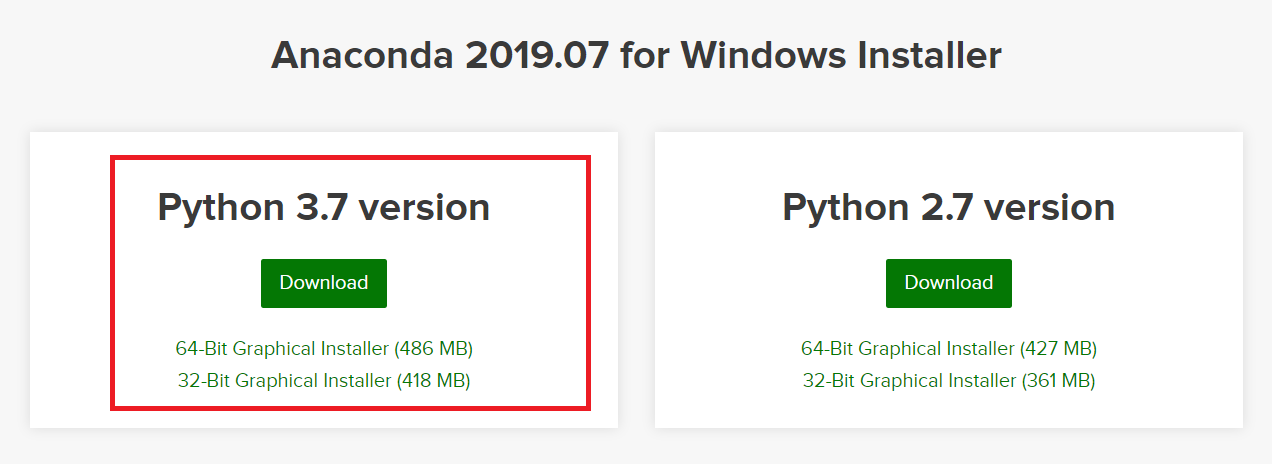
\includegraphics[scale=0.5]{figure/chapter1/anaconda2.png}
\end{figure}

下载完毕后,双击 exe 文件安装,安装过程参照下图:


\begin{figure}[!ht]
  \centering
  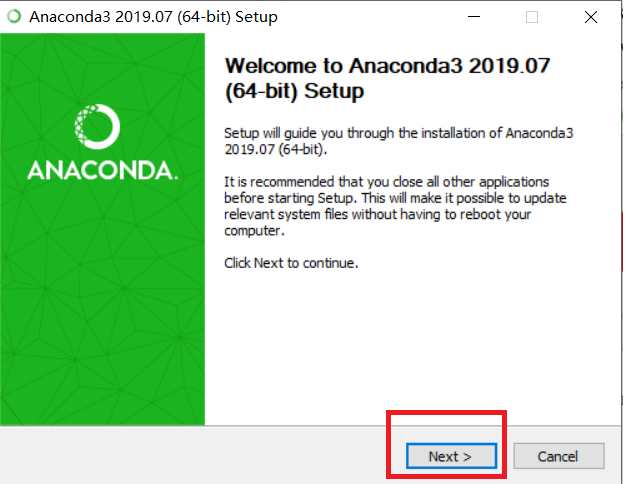
\includegraphics[scale=0.5]{figure/chapter1/anaconda7.png}\quad
  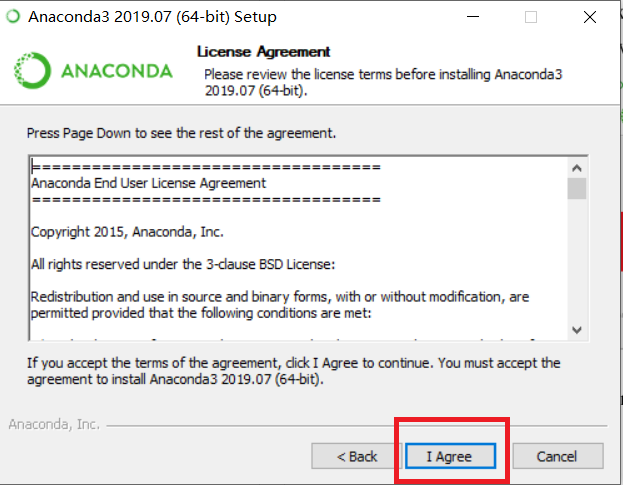
\includegraphics[scale=0.5]{figure/chapter1/anaconda8.png}
\end{figure}

安装目录默认的是 C 盘,可以通过点击 Browse 更改为自定义位置。


\begin{figure}[!ht]
  \centering
  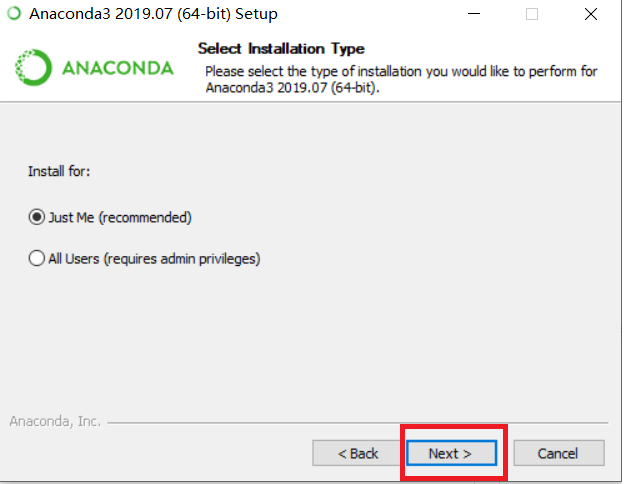
\includegraphics[scale=0.5]{figure/chapter1/anaconda9.png}\quad
  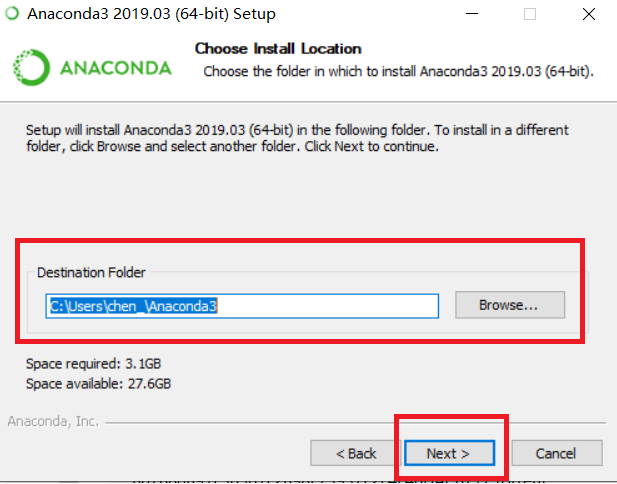
\includegraphics[scale=0.5]{figure/chapter1/anaconda3.png}
\end{figure}

\begin{figure}[!ht]
  \centering
  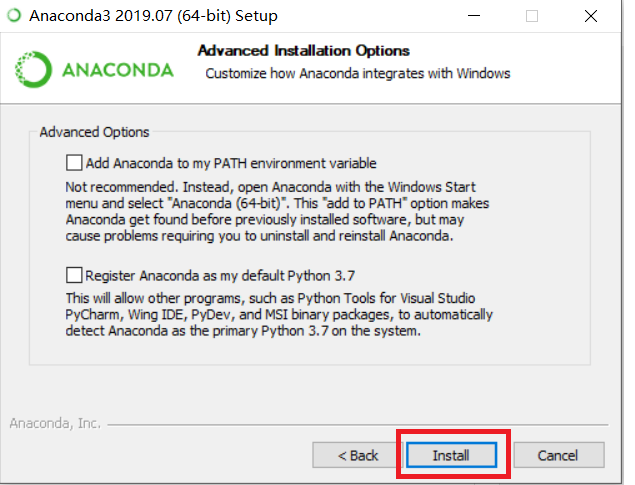
\includegraphics[scale=0.5]{figure/chapter1/anaconda10.png}\quad
  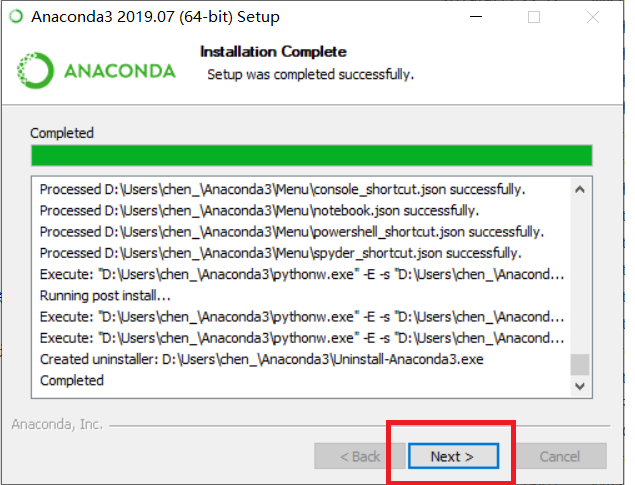
\includegraphics[scale=0.5]{figure/chapter1/anaconda12.png}
\end{figure}

\begin{figure}[!ht]
  \centering
  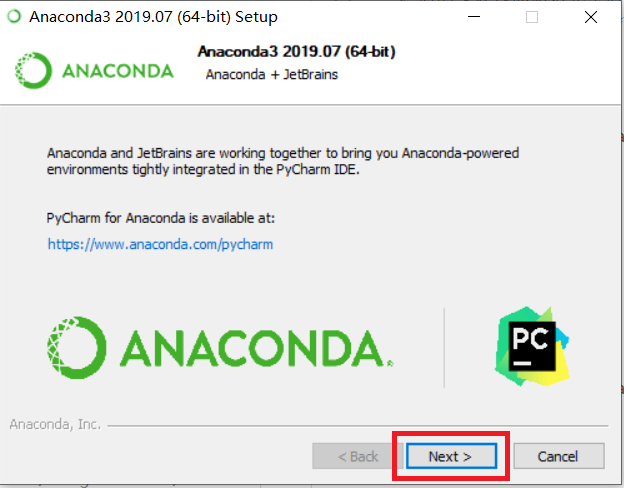
\includegraphics[scale=0.5]{figure/chapter1/anaconda13.png}\quad
  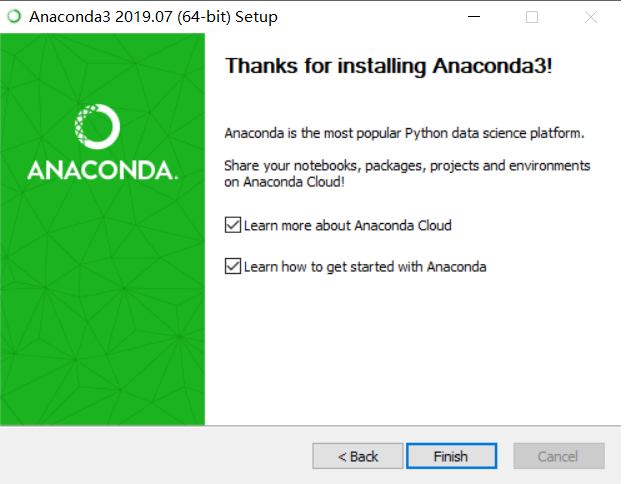
\includegraphics[scale=0.5]{figure/chapter1/anaconda14.png}
\end{figure}

安装完毕后,在 Windows 菜单栏里找到名为“Anaconda-Navigator”的图标,点击打开 Anaconda。

\begin{figure}[!ht]
  \centering
  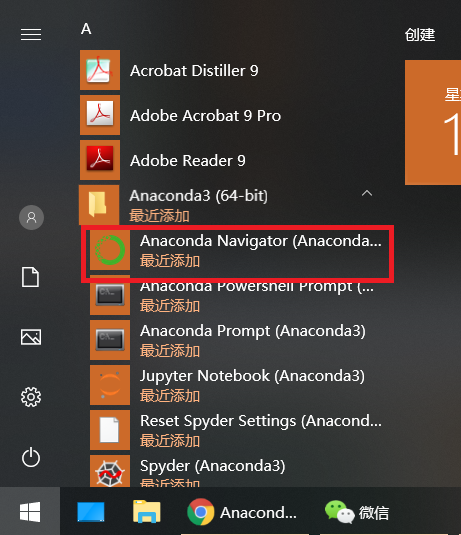
\includegraphics[scale=0.5]{figure/chapter1/anaconda11.png}
\end{figure}


启动(Launch) Spyder,就能够编译 Python 了。

\begin{figure}[!ht]
  \centering
  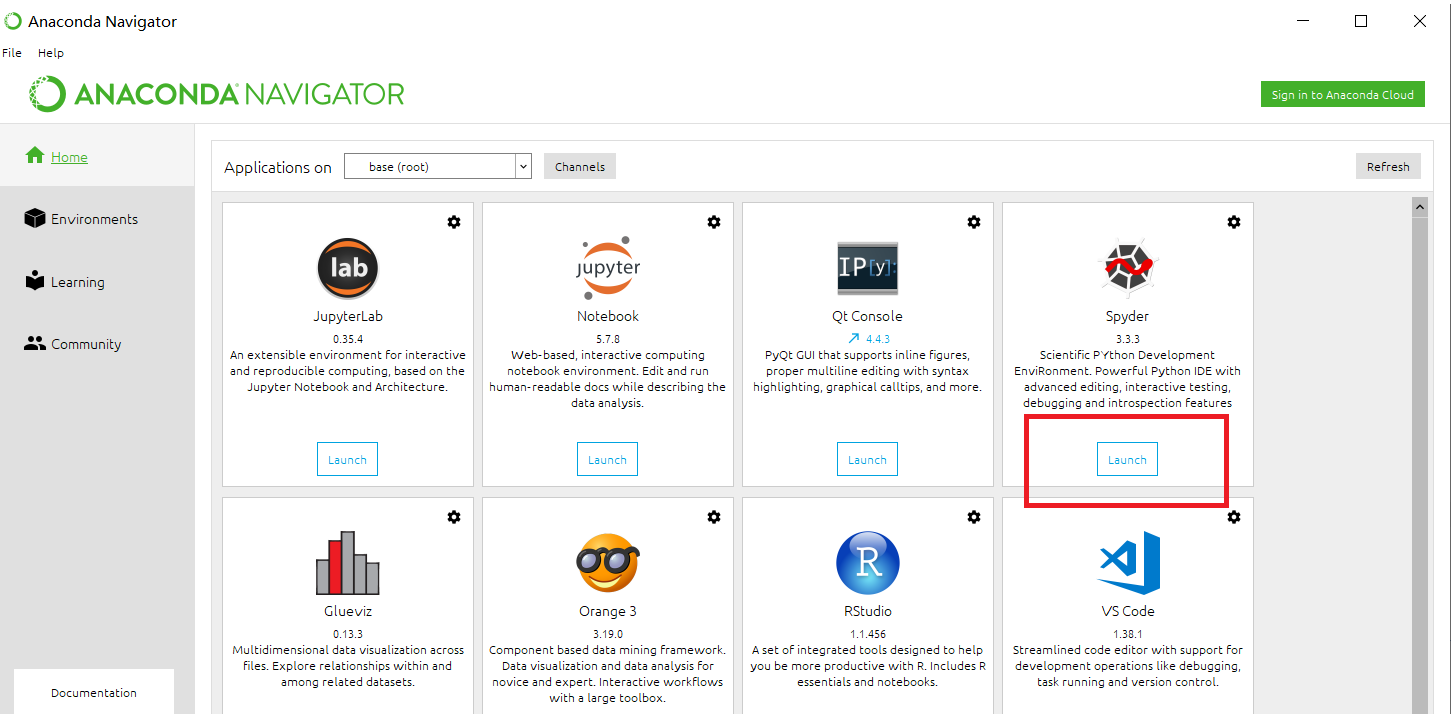
\includegraphics[scale=0.3]{figure/chapter1/anaconda4.png}
\end{figure}


Spyder 的界面非常类似 Matlab,交互式工具 IPython console 就在窗口界面中。我们在 IPython 中输入 print(`Hello world'),目的是让 Python 把 Hello World 打印到屏幕上,测试 Spyder的运行。

\begin{figure}[!ht]
  \centering
  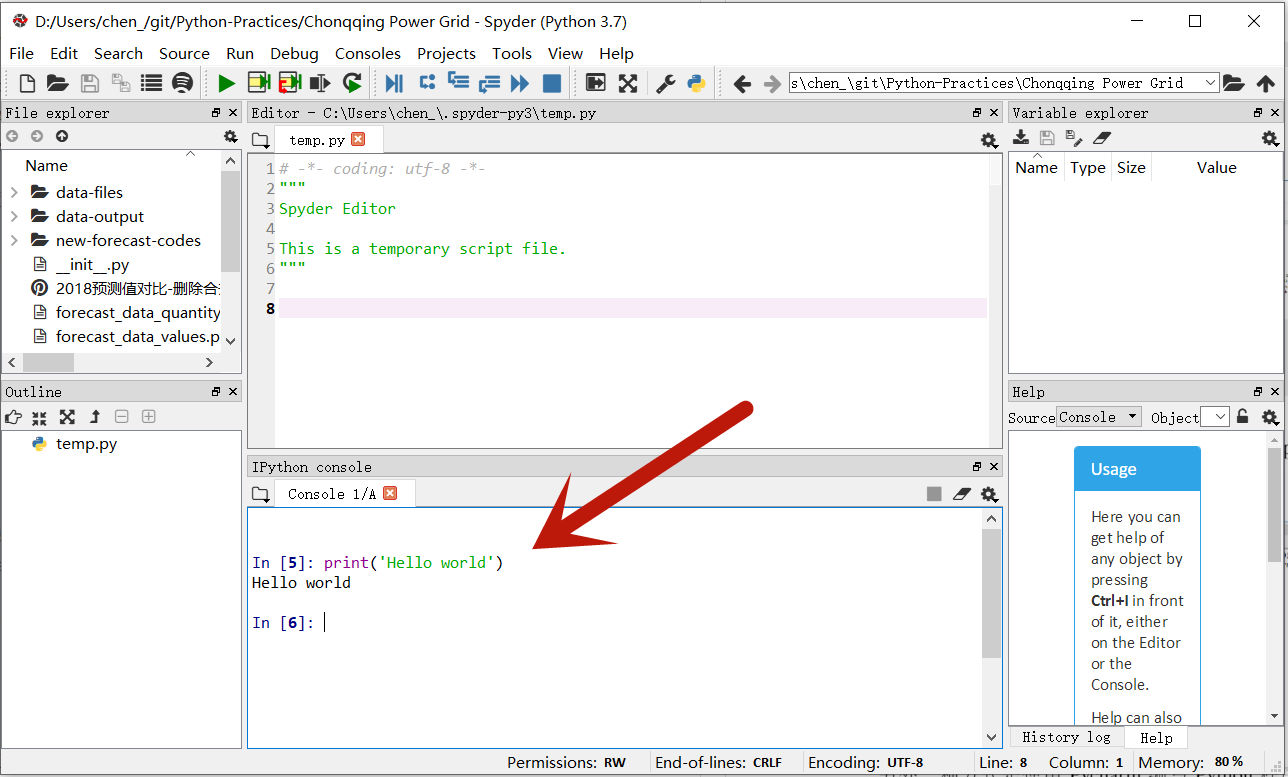
\includegraphics[scale=0.4]{figure/chapter1/anaconda5.png}
\end{figure}



\subsection{Python + Pycharm}

另外一种方式是使用 Pycharm 编写 Python 程序,但由于 Pycharm 并不自带 Python,我们还需要专门把 Python 下载下来。

\subsubsection{下载Python}

Python 的官方网址为:\href{https://www.Python.org}{https://www.Python.org}。打开网址后,从 Download 里面可以找到不同操作系统的 Python 版本下载。下面我们以 Windows 系统为例讲述 Python 的安装。

\begin{figure}[!ht]
  \centering
  \includegraphics[scale=0.6]{figure/chapter1/PythonDownload.png}
\end{figure}

下载完成后,双击 exe 文件安装,切记要勾选 Add Python 3.7 to PATH, 然后点击 Install Now(默认安装目录,默认安装 pip 等)或 Customize installation(可以自己设置安装目录等),我们选择 Customize installation。

\begin{figure}[ht]
  \centering
  \includegraphics[scale=0.4]{figure/chapter1/PythonDownload2.png}\quad
  \includegraphics[scale=0.4]{figure/chapter1/PythonDownload4.png}
\end{figure}

\clearpage
\begin{figure}[ht]
  \centering
  \includegraphics[scale=0.4]{figure/chapter1/PythonDownload5.png}\quad
  \includegraphics[scale=0.4]{figure/chapter1/PythonDownload6.png}
\end{figure}

为了测试 Python 是否安装成功,打开命令行窗口(win10 系统中敲 win 健,再输入 cmd,然后回车),输入 Python -{}-version(注意是两个短横线),若能显示 Python 的版本信息,则代表 Python 已正确安装。

\begin{figure}[!ht]
  \centering
  \includegraphics[scale=0.7]{figure/chapter1/PythonDownload3.png}
\end{figure}

\subsubsection{下载 Pycharm}


Pycharm 的官方网址:\href{http://www.jetbrains.com/pycharm}{http://www.jetbrains.com/pycharm},点击 DOWNLOAD 开始安装。

\begin{figure}[!ht]
  \centering
  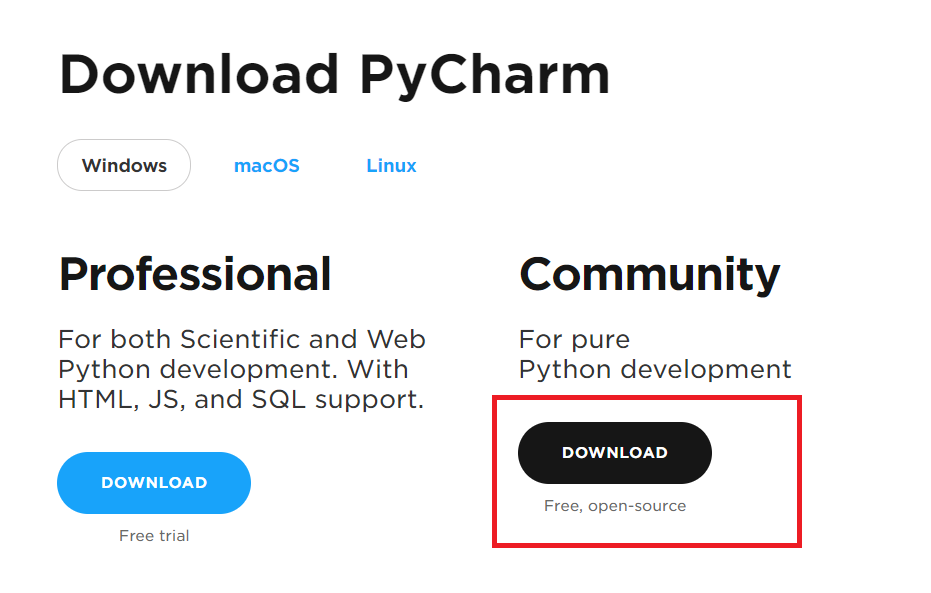
\includegraphics[scale=0.6]{figure/chapter1/pycharm.png}
\end{figure}

一般选择免费版本下载,下载完成后双击 exe 进行安装。

\clearpage
\begin{figure}[!ht]
  \centering
  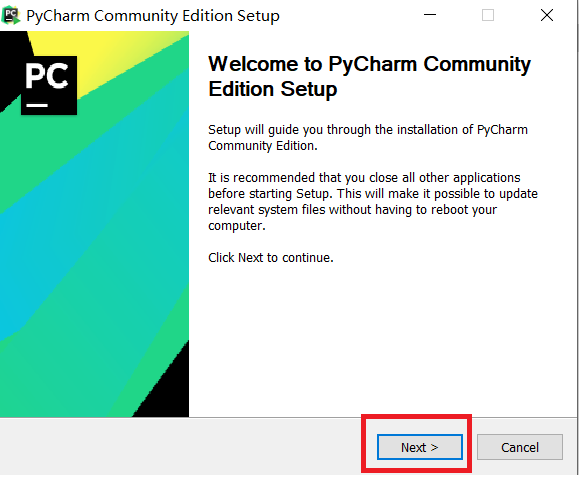
\includegraphics[scale=0.5]{figure/chapter1/pycharm5.png}\quad
  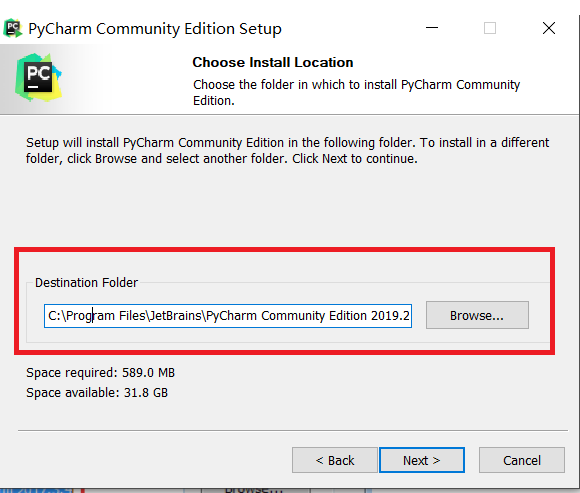
\includegraphics[scale=0.5]{figure/chapter1/pycharm2.png}
\end{figure}

可以通过图中的 Browse 更改安装目录,其他步骤按照默认设置即完成安装。
\begin{figure}[!ht]
  \centering
  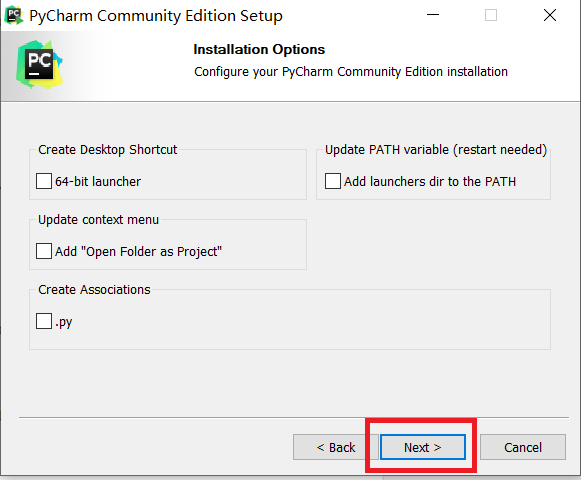
\includegraphics[scale=0.5]{figure/chapter1/pycharm6.png}\quad
  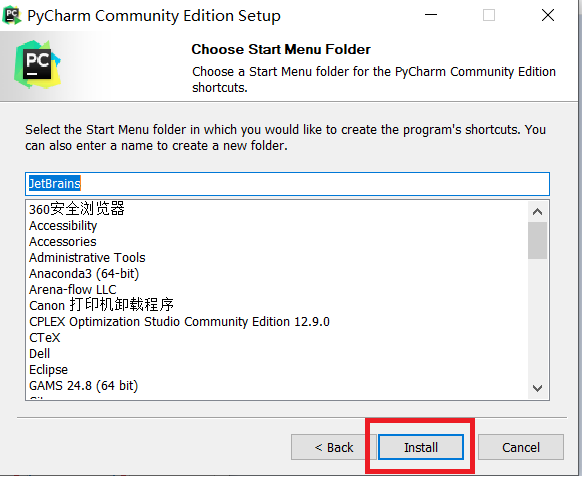
\includegraphics[scale=0.5]{figure/chapter1/pycharm7.png}
\end{figure}

\begin{figure}[!ht]
  \centering
  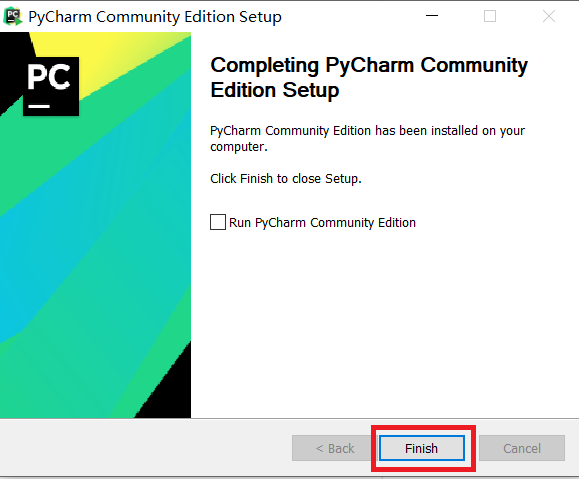
\includegraphics[scale=0.5]{figure/chapter1/pycharm8.png}
\end{figure}


完成安装后,从 Windows 菜单栏里找到 jetbrains Pycharm,点击打开 Pycharm。

\begin{figure}[!ht]
  \centering
  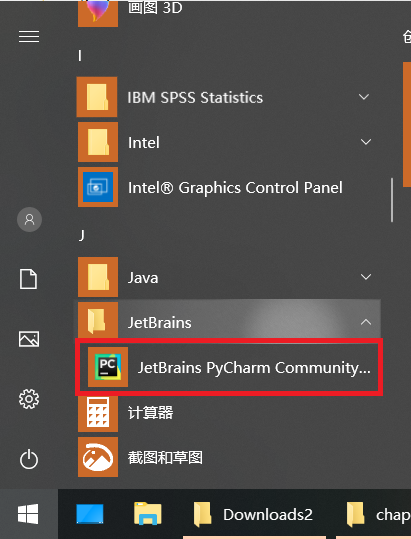
\includegraphics[scale=0.4]{figure/chapter1/pycharm9.png}
\end{figure}

之后的设置如下面的图所示:

\begin{figure}[!ht]
  \centering
  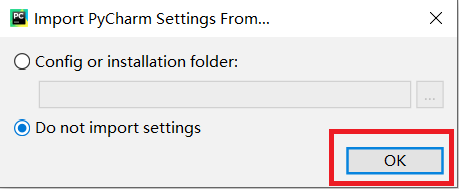
\includegraphics[scale=0.8]{figure/chapter1/pycharm10.png}
\end{figure}

\begin{figure}[!ht]
  \centering
  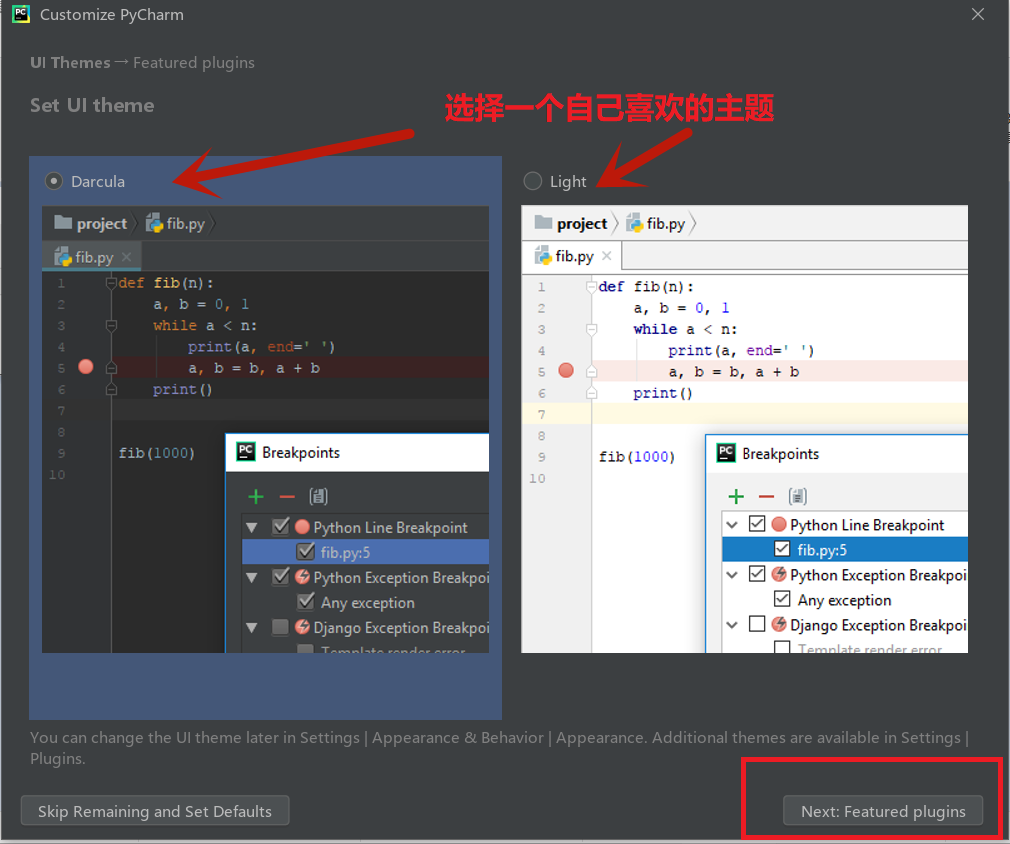
\includegraphics[scale=0.3]{figure/chapter1/pycharm11.png}\quad
  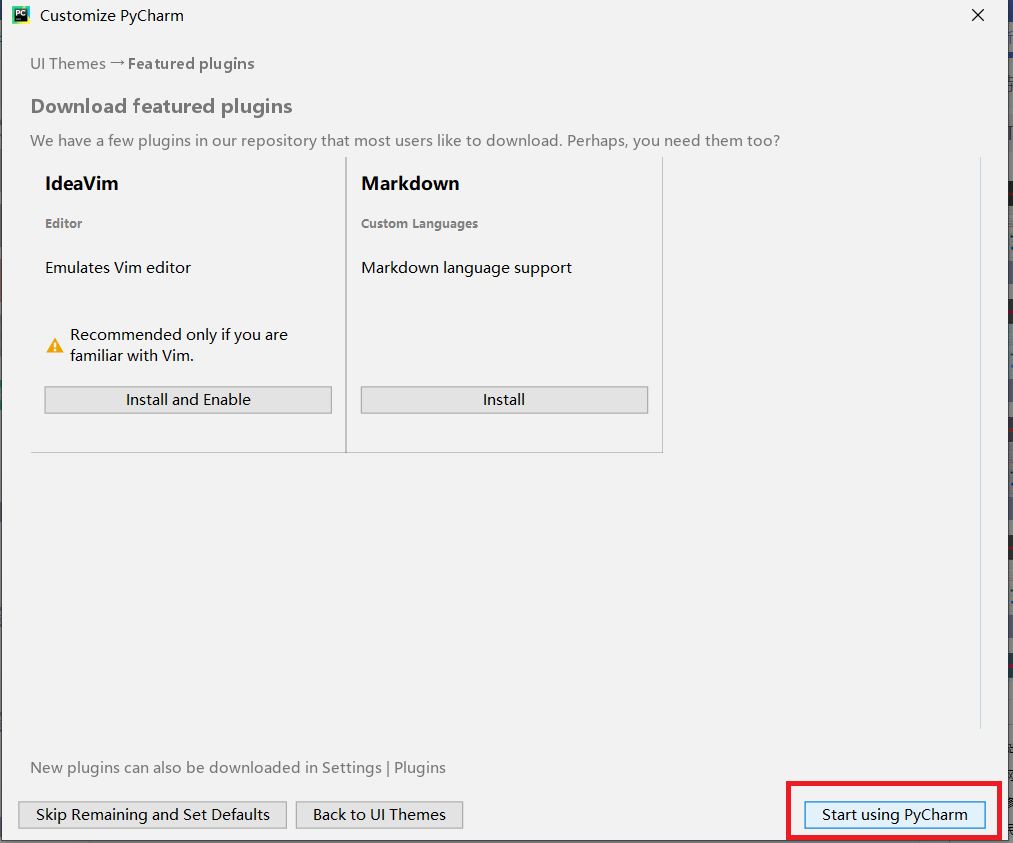
\includegraphics[scale=0.3]{figure/chapter1/pycharm12.png}
\end{figure}

点击 Create New Project,创建一个新项目,项目的地址以及名字可以自己替换。

\begin{figure}[!ht]
  \centering
  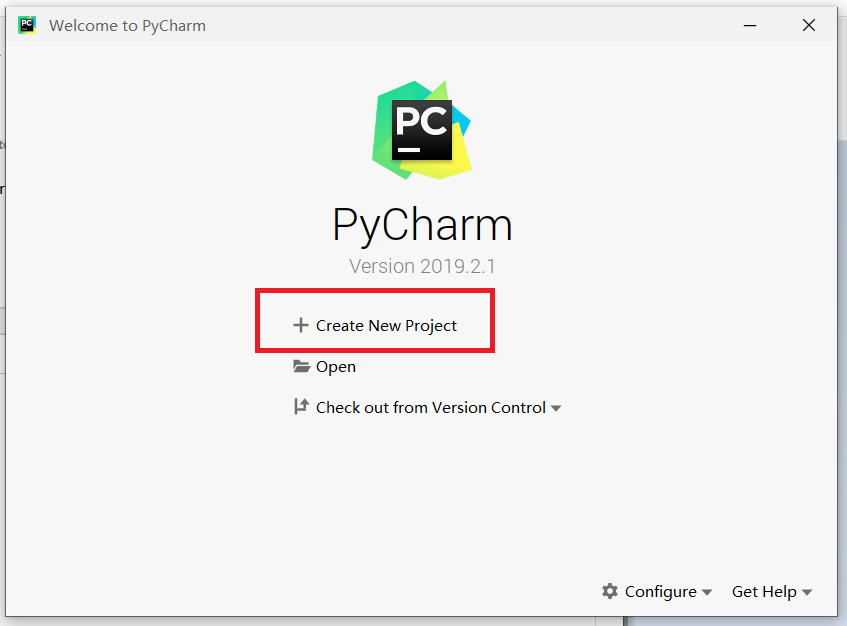
\includegraphics[scale=0.4]{figure/chapter1/pycharm13.png}\quad
  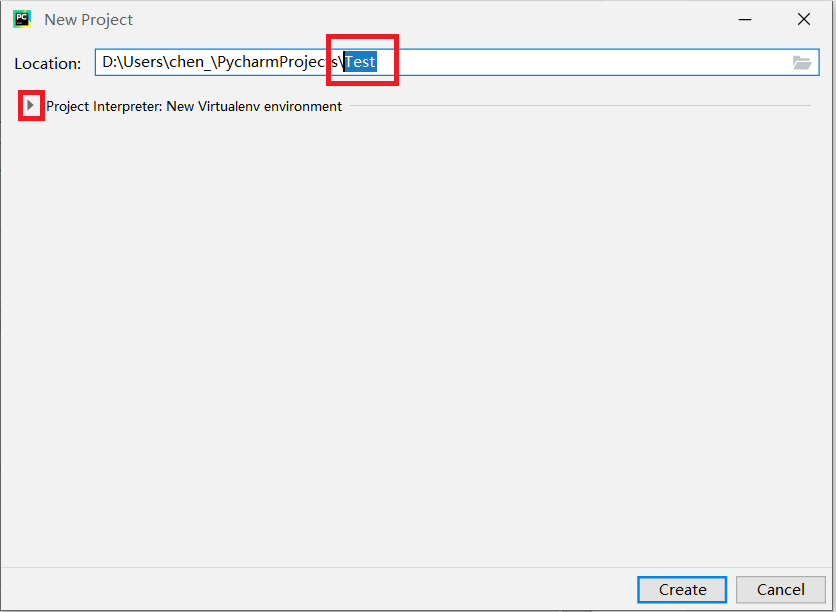
\includegraphics[scale=0.4]{figure/chapter1/pycharm14.png}
\end{figure}

% 点击这个三角符号,可以看到 Pycharm 已经自动获取了我们安装的 Python 版本。
%
%


为了测试 Pycharm 是能安装成功,可以点击 Pycharm 界面最下面的 Python Console,打开控制台(Python Console 是一个交互式的 Python 编辑器,可以快速运行一些指令,一般调试时用),输入一条 Python 指令:print(`Hello World'),若能正确运行,则表示 Pycharm 安装成功了。

\clearpage

\begin{figure}[!ht]
  \centering
  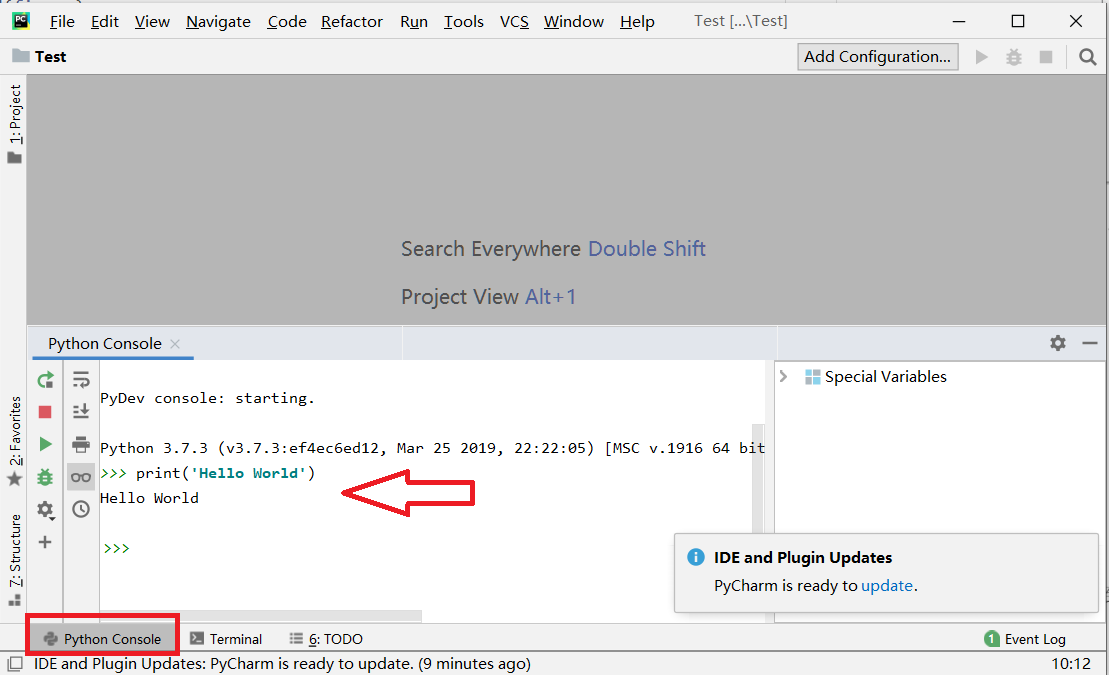
\includegraphics[scale=0.4]{figure/chapter1/pycharm4.png}
\end{figure}

有时候可能提醒我们设置 Pycharm 中的 Python 解释器。设置方式如下:依次点击 file--settings--project interpreter,将 interpreter 设置为我们 Python 安装路径中的 Python.exe(笔者电脑的位置为 \path{D:\Python:\Python.exe})。

\begin{figure}[!ht]
  \centering
  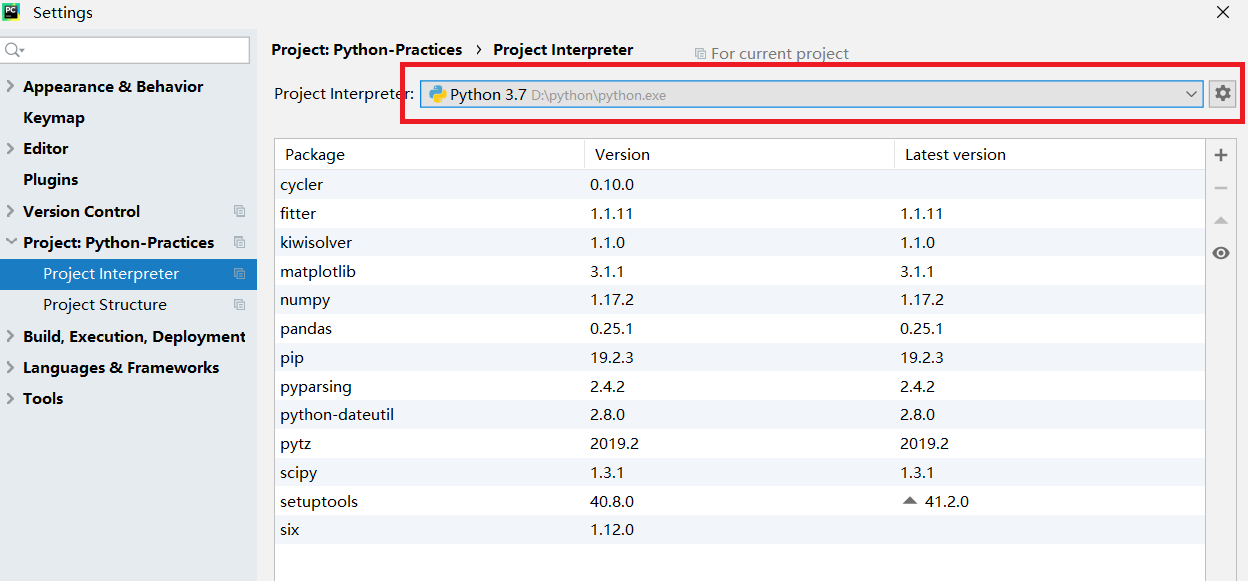
\includegraphics[scale=0.4]{figure/chapter1/pycharm3.png}
\end{figure}

我们可以在刚刚新建的项目(project)中新建一个 Python 文件,操作步骤如下图所示:

\begin{figure}[!ht]
  \centering
  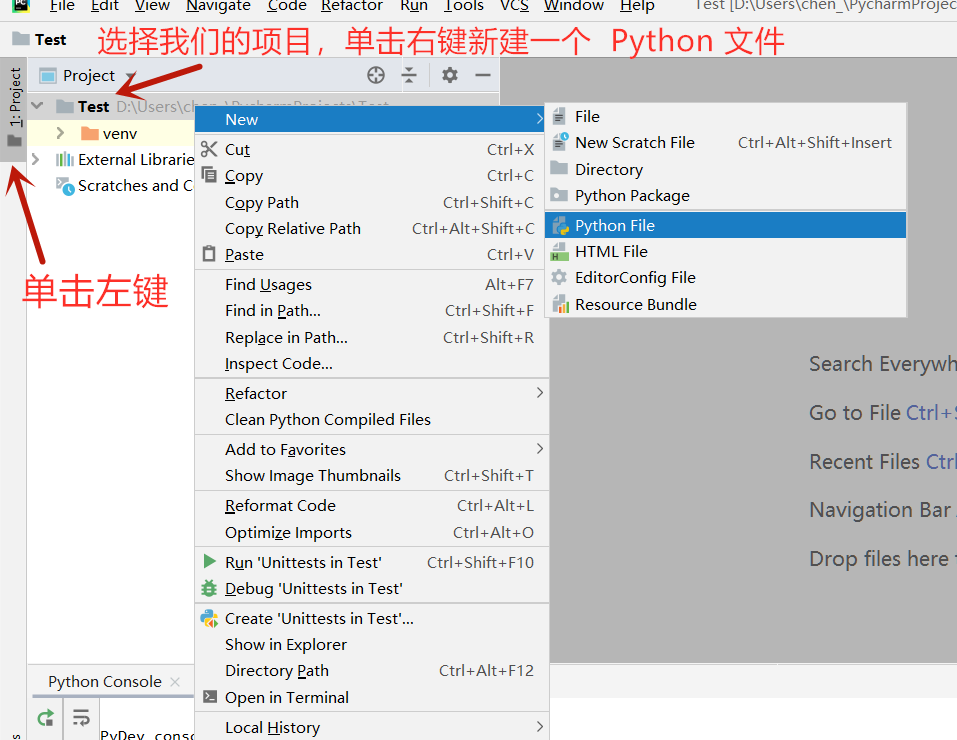
\includegraphics[scale=0.5]{figure/chapter1/pycharm15.png}
\end{figure}

命名 Python 文件的名字:

\begin{figure}[!ht]
  \centering
  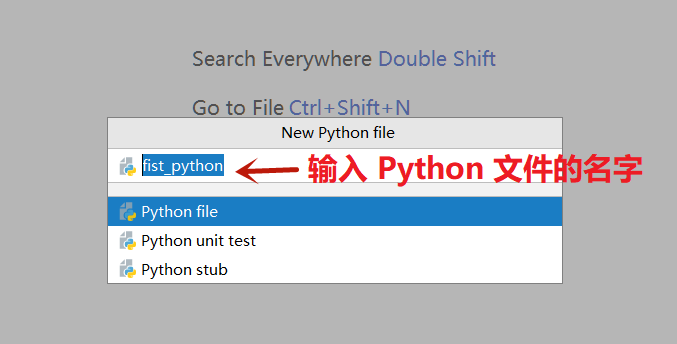
\includegraphics[scale=0.6]{figure/chapter1/pycharm16.png}
\end{figure}

输入代码后,在空白处单击右键,选择 run 运行程序:

\begin{figure}[!ht]
  \centering
  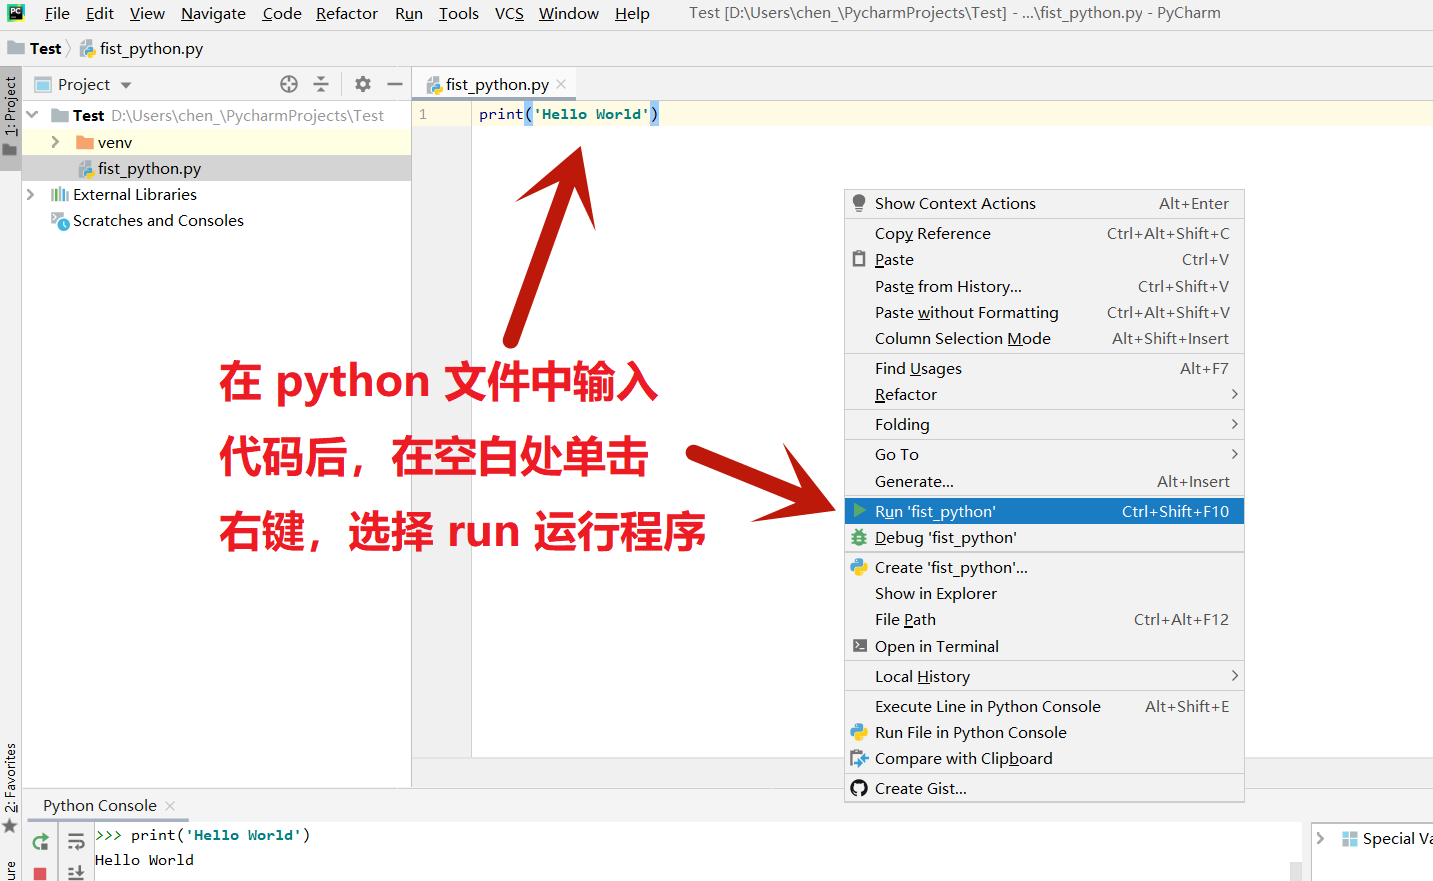
\includegraphics[scale=0.4]{figure/chapter1/pycharm17.png}
\end{figure}

在 Pycharm 下面的窗口中,就能看到运行输出的文字:

\begin{figure}[!ht]
  \centering
  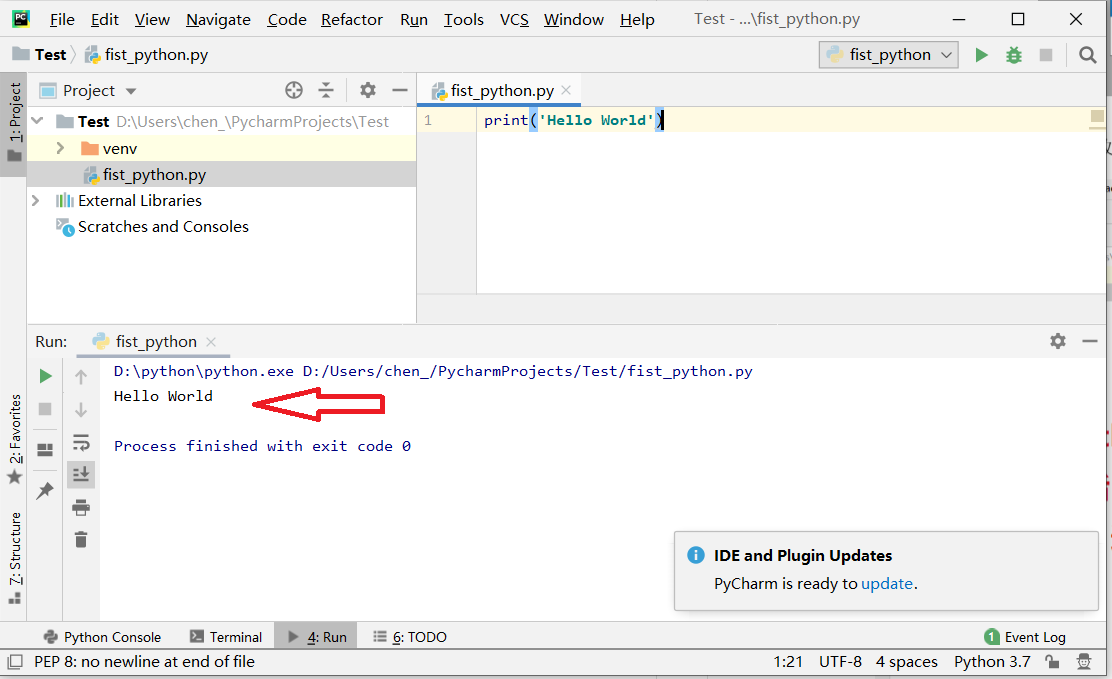
\includegraphics[scale=0.5]{figure/chapter1/pycharm18.png}
\end{figure}

\clearpage
\section{数据分析常用 Python 工具包的安装}

Python 的最大优势在于它有很多第三方开发的包,能够实现各种各样的功能。若我们使用 Anaconda,一般可以通过 conda 工具安装。若我们使用 Pycharm,一般用 pip 工具进行安装。

数据分析的常用包有:

\vspace{5pt}
\begin{itemize}
  \item numpy --- 用于数组和矩阵操作

  \item pandas --- 用于处理表格数据,数据分析的重要工具

  \item matplotlib --- 常用的基础绘图包

  \item seaborn --- 另外一个绘图包

  \item scipy --- 科学计算包,包括一些基础的统计学

  \item statsmodels --- 统计建模与分析包

  \item sklearn --- 机器学习包

  %\item xlrd --- 用于读取 excel 数据

  %\item openpyxl --- 用于存储 pandas 数据到 excel


\end{itemize}
\vspace{5pt}

\subsection{用 Anaconda 安装}

Anaconda 已经默认帮我们安装了很多常用的包,很多时候并不需要我们再安装新包。若实在有必要,可以通过 Anaconda 自带的 Conda 工具安装。方法是:在 Windows 菜单栏里,点击 Anaconda Prompt,打开 Anaconda 的命令行窗口,如下图所示:

\begin{figure}[!ht]
  \centering
  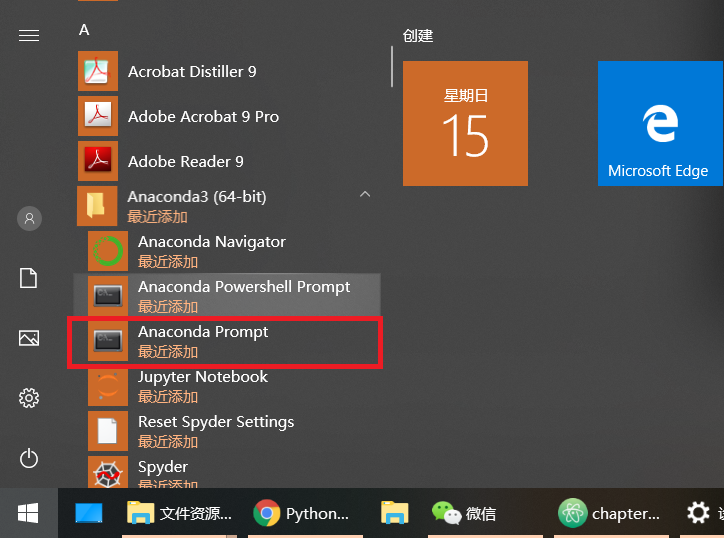
\includegraphics[scale=0.4]{figure/chapter1/anaconda6.png}
\end{figure}

常用的 conda 语法如下:

\begin{center}
\begin{tcolorbox}[title = conda 的常用语法]
  \centering\bf
  \begin{tcboutputlisting}
  \begin{tabular}{>{\bfseries}ll}
    安装包:&conda install [package\_name]\\
    搜索包:&conda search [package\_name]\\
    卸载包:&conda uninstall [package\_name]\\
    更新包: & conda install [package\_name] -U\\
  显示已安装包列表: &conda list
  \end{tabular}
\end{tcboutputlisting}
\end{tcolorbox}
\end{center}

例如,安装 numpy 包的命令输入为:conda install numpy。不过,国内用 conda 安装包时的网速有时候比较慢。

\subsection{用 pip 安装}
pip 是 Python 包管理工具,该工具提供了对 Python 包的查找、下载、安装、卸载的功能。在我们安装 Python 时, pip 也是自动安装的,并且 pip 的地址已经添加到了计算机的环境变量里了。 打开命令行窗口(win10 系统中敲 win 健,再输入 cmd,然后回车),输入 pip (有时候若电脑里其他软件也内置 pip,则需要输入 pip.exe才能正确显示)回车,若能显示如下图所示的很多内容,则表示 pip 已经成功安装了。

\begin{figure}[!ht]
  \centering
  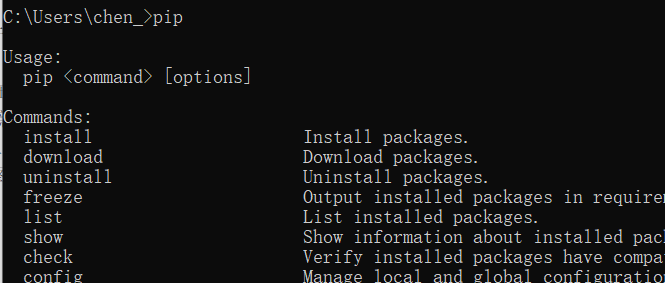
\includegraphics[scale=0.6]{figure/chapter1/pip.png}
\end{figure}

常用的 pip 语法如下:

\begin{center}
\begin{tcolorbox}[title = pip 的常用语法]
  \centering\bf
  \begin{tcboutputlisting}
  \begin{tabular}{>{\bfseries}ll}
    安装包:&pip install [package\_name]\\
    搜索包:&pip search [package\_name]\\
    卸载包:&pip uninstall [package\_name]\\
    更新包: & pip install [package\_name] -U\\
  显示已安装包列表: &pip list
  \end{tabular}
\end{tcboutputlisting}
\end{tcolorbox}
\end{center}

例如,安装 numpy 包时在命令行窗口输入 pip install numpy,操作命令与运行结果如下图。
\begin{figure}[!ht]
  \centering
  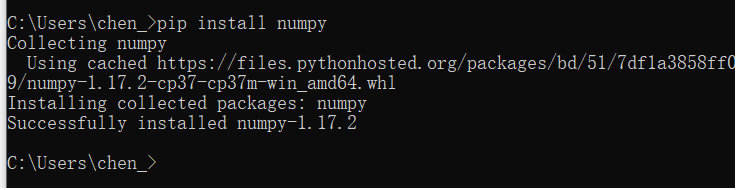
\includegraphics[scale=0.6]{figure/chapter1/pip2.png}
\end{figure}



因此,我们可以在命令行窗口,利用 pip 的安装命令将其他包安装到 Python 中。

\begin{lstlisting}
pip install pandas
pip install xlrd
pip install openyxl
pip install matplotlib
pip instal scipy
pip install statsmodels
pip install seaborn
\end{lstlisting}

% \chapter{Python 的操作基础}

\section{Python 中定义函数}

\section{Python 的常用数据类型}

\section{Python 的常用数据结构}

% \chapter{Python 中的 Numpy 与 Pandas}

\section{Numpy 的常用操作}

\clearpage
\section{Pandas 的常用操作}

Pandas 是 Python 做统计分析时最重要的数据分析工具之一,它基于 Numpy 开发,提供了许多处理大型数据集所需的函数,可以灵活高效的处理各种数据集。

Pandas 一般使用两种数据类型:DataFrame 和 Series。其中 DataFrame 是二维数据,而 Series 是一维数据。可以这样简单理解:DataFrame 相当于 Excel 里面的一张表,而 Series 是表中的某一列。还有一个表示三维数据的类型 Panel,但我们经常使用的是前面两种数据类型。使用 Pandas 时首先到导入 pandas 包。

\begin{lstlisting}[Language=Python]
import pandas as pd
\end{lstlisting}

\subsection{创建、读取和存储数据}

\subsubsection{创建}
 例如有下面的数据:

 \begin{table}[!ht]
 \centering
 \renewcommand{\arraystretch}{1.2}
 \begin{tabular}{|l|l|l|l|}
 \hline
 &统计学 & 高数 & 英语 \\ \hline
 张三 & 85 & 82 & 84 \\ \hline
 李四 & 68 & 63 & 90 \\ \hline
 王五 & 90 & 88 & 78 \\ \hline
 \end{tabular}
 \end{table}

我们可以使用下面的代码读取到一个 DataFrame 里面:

\begin{lstlisting}[Language=Python]
df = pd.DataFrame({'统计学': [85, 68, 90], '高数': [82, 63, 88], '英语': [84, 90, 78]}, index=['张三', '李四', '王五'])
print(df)
\end{lstlisting}

从上面可以看出,DataFrame 通过一个字典类型设置各列的标题及对应数值,通过一个 index 数组设置行标题。还有一种方式是通过 numpy 的 array 数组设置数值,然后通过 columns 数组设置列标题,通过 index 数组设置行标题\footnote{如果创建时不设置行标题或列标题,系统会自动生成从 0 到行数或列数的数组作为标题}:

\begin{lstlisting}[Language=Python]
import numpy as np

df = pd.DataFrame(np.array([[85, 68, 90], [82, 63, 88], [84, 90, 78]]), columns=['统计学', '高数', '英语'], index=['张三', '李四', '王五'])
print(df)
\end{lstlisting}

一个 DataFrame 包括 columns(列标题),index(行标题)与 values(数值)三个部分,上述例子中的 columns, index,values 如下图所示:

\begin{figure}[!ht]
\centering
  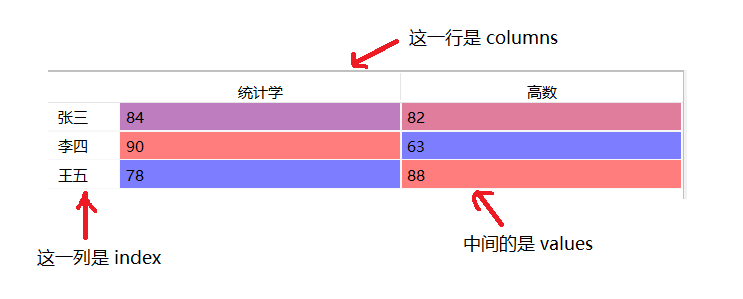
\includegraphics{figure/chapter2/pandas.png}
\end{figure}

\subsubsection{读取}
大部分情况下,我们要读取 Excel 里面的数据,假设上面的例子在 excel 文件 '成绩数据.xlsx' 并放在电脑硬盘某个位置:

\begin{figure}[!ht]
\centering
  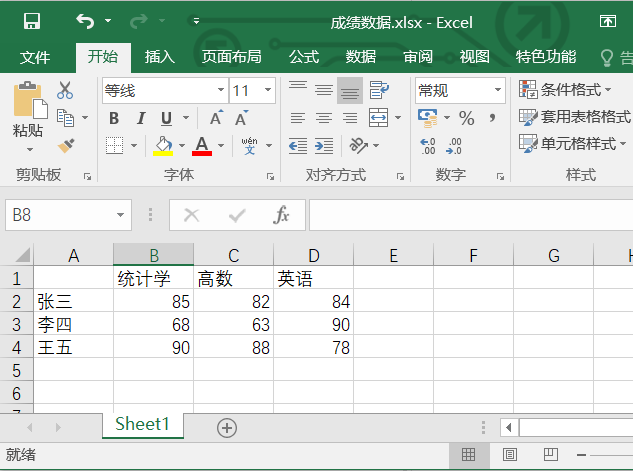
\includegraphics[scale=0.7]{figure/chapter2/pandas2.png}
\end{figure}

可以通过下面的代码读取文件:

\begin{lstlisting}[Language=Python]
df = pd.read_excel(r'D:\Users\chen_\git\Statistics-book\datas\成绩数据.xlsx', index_col=0)
\end{lstlisting}

数据文件的地址位于 \path{`D:\Users\chen_\git\Statistics-book\datas\成绩数据.xlsx'},使用 read\_excel 时\textbf{在文件位置字符串前面加上字母 r},这样 python 就能找到我们的数据文件了。index\_col=0 表示行标题位于第一列(不然 read\_excel 会把第一列内容读取到 values 里面,并默认 index 为 0, 1, 2, \dots)。read\_excel 会自动将 Excel 第一行的内容作为行标题。read\_excel 的一般语法为:

\begin{center}
\begin{tcolorbox}[title = read\_excel 函数的语法]
\textbf{read\_excel(io, sheetname=0, header=0, skiprows=None,  index\_col=None)}
\tcblower
\vspace{10pt}

\begin{tcboutputlisting}
\begin{tabular}{>{\bfseries}ll}
  io &数据文件的地址与名字,一般为字符串\\
  sheetname & 工作簿名字,默认为0,表示读取第一张工作簿\\
header &作为列名的行,默认为0,即取第一行的值为列名\\
skiprows&省略指定行数的数据,从第一行开始查起\\
index\_col&行标题所在的列\\
\end{tabular}
\end{tcboutputlisting}
\tcbuselistingtext

\end{tcolorbox}
\end{center}

\sloppy
更多的语法设置可以查看官网文档:

\href{https://pandas.pydata.org/pandas-docs/version/0.20/generated/pandas.read\_excel.html}{https://pandas.pydata.org/pandas-docs/version/0.20/generated/pandas.read\_excel.html}

还有一种常见的数据文件类型为 csv,我们只需使用 pandas 中的函数 read\_csv,它的语法与 read\_excel 基本一样。但是, read\_csv 可以读取网络数据库中的 csv 文件,例如下面的例子显示世界上所有国家与所属的大洲。

\begin{lstlisting}[Language=Python]
df = pd.read_csv('https://raw.githubusercontent.com/cs109/2014_data/master/countries.csv')
print(df)
\end{lstlisting}

\begin{figure}[!ht]
\centering
  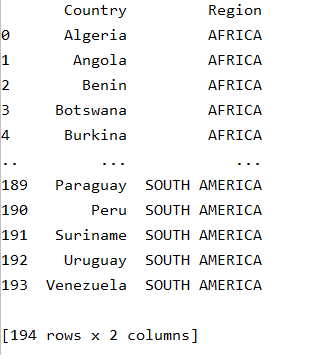
\includegraphics[scale=0.7]{figure/chapter2/pandas7.png}
\end{figure}
\subsubsection{存储}

存储时使用函数 to\_excel 或 to\_csv。例如我们将 DataFrame 存储到 \path{E:\datas} 文件夹里,并命名为 marks.xlsx:

\begin{lstlisting}[Language=Python]
import pandas as pd
import numpy as np

df = pd.DataFrame(np.array([[85, 68, 90], [82, 63, 88], [84, 90, 78]]), columns=['统计学', '高数', '英语'], index=['张三', '李四', '王五'])
df.to_excel(r'E:datas\marks.xlsx')
\end{lstlisting}

在上面的代码中,若直接写成 df.to\_excel('marks.xlsx'),则文件存储的路径为当前工作环境所在的文件夹。


\subsection{查看数据}

\subsubsection{概览数据}
快速查看 DataFrame 各列数据的统计信息可以使用 discribe() 函数,包括各列数据的非空数值数目、均值、标准差、最大值、最小值、分位数。例如上面的例子:

\begin{lstlisting}[Language=Python]
df.describe()
\end{lstlisting}

\begin{figure}[!ht]
\centering
  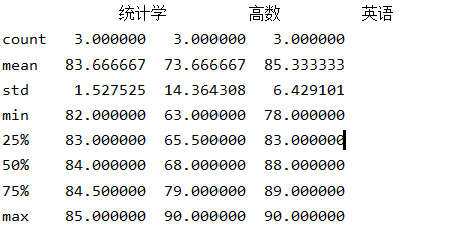
\includegraphics[scale=0.7]{figure/chapter2/pandas3.png}
\end{figure}

info() 函数可以查看各列数据的类型:

\begin{lstlisting}[Language=Python]
df.info()
\end{lstlisting}

\begin{figure}[!ht]
\centering
  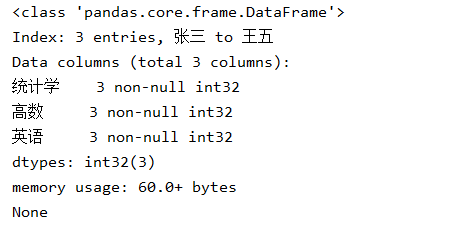
\includegraphics[scale=0.8]{figure/chapter2/pandas4.png}
\end{figure}

DataFrame 的 sample() 函数可以从数据中随机抽取样本,小括号中用数字表示抽取的样本个数。例如,下面的代码从 df 里面随机抽取 2 个样本:
\begin{lstlisting}[Language=Python]
df.sample(2)
\end{lstlisting}

\begin{figure}[!ht]
\centering
  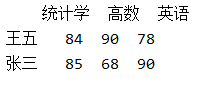
\includegraphics[scale=0.8]{figure/chapter2/pandas8.png}
\end{figure}

另外,head() 函数可以显示 DataFrame 前五行数据,而 tail() 函数可以显示 DataFrame 最后五行数据。

\subsubsection{查看单列、单行、单元格数据}

查看某一列数据时,最简单的方式是中括号里面输入列名的方式,例如查看英语成绩那一列数据:
\begin{lstlisting}[Language=Python]
df['英语']
\end{lstlisting}

\begin{figure}[!ht]
\centering
  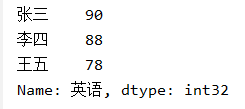
\includegraphics[scale=0.8]{figure/chapter2/pandas5.png}
\end{figure}

查看某一行数据时,最简单的方式是中括号里面输入行名方式,例如查看张三哪一行的数据:
\begin{lstlisting}[Language=Python]
df['张三']
\end{lstlisting}

也可以用中括号里面跟着行索引的方式(行数 : 行数 + 1),即 df[0:1],与上面代码显示效果一样。


\begin{figure}[!ht]
\centering
  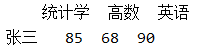
\includegraphics[scale=0.8]{figure/chapter2/pandas6.png}
\end{figure}


若查看某个单元格,比较方便的方式是用两个中括号,每个中括号内分别跟着行名和列名,例如查看张三的高数成绩:
\begin{lstlisting}[Language=Python]
df['张三']['高数']  # 显示张三的高数成绩为 68
\end{lstlisting}



\subsubsection{查看多列、多行数据 iloc}

查看多行、多列数据时,一般用 iloc 比较方便,而且 iloc 不仅能查看多行多列数据,也能查看单行、单列或某个单元格数据:

例如,查看行:

\begin{lstlisting}[Language=Python]
df.iloc[1]          # 查看第 2 行数据
df.iloc[0:2]        # 查看前 2 行数据
df.iloc[[0, 2]]     # 查看第 1 行与第 3 行数据
\end{lstlisting}

查看列:

\begin{lstlisting}[Language=Python]
df.iloc[:, 1]       # 查看第 2 列数据
df.iloc[:, 0:2]     # 查看前 2 列数据
df.iloc[:, [0, 2]]  # 查看第 1 列与第 3 列数据
\end{lstlisting}

查看一块数据:
\begin{lstlisting}[Language=Python]
df.iloc[0:2, 0:2]          # 查看前 2 行,前 2 列的一块数据
df.iloc[[0, 2],  [0, 2]]   # 查看第 1、第 3 行,第 1、第 3 列的一块数据
df.iloc[0:2, [0, 2]]       # 查看前 3 行,第 1、第 3 列的一块数据
df.iloc[[0, 2], 0:2]       # 第 1、第 3 行,前 2 列的一块数据
\end{lstlisting}

查看某个单元格:
\begin{lstlisting}[Language=Python]
df.iloc[1, 1]   # 查看第 2 行,第 2 列的单元格数据
\end{lstlisting}

\subsection{增加、删除、修改、查询数据}

\subsection{数据合并}

\subsection{数据排序}

\subsection{分组汇总数据}

\section{数据的概括性度量}

%  \chapter{统计数据的图形描述}

使用图形描述统计结果是应用统计的基本技能之一。人类在接受信息时,大脑皮层总是优先提取可视化的图形,其次才是具体的文字内容。一些漂亮的图形会使得读者或观众迅速得知我们想要表达的信息。因此不论是写论文,还是汇报展示,做到图文并茂非常重要。

由于 Python 具有良好的可扩展性,它在画图方面具有大量的绘图包。本章将展示如何用 Python 的 matplotlib 工具包、pandas工具包、seaborn 工具包来画出各种各样的统计图形。三个工具包在画图方面的简单比较如下:

\begin{itemize}
  \item matplotlib 是一个比较传统的画图包
  \item pandas 画图其实是调用了matplotlib,因此显示效果与参数设置与 matplotlib 画图差不多
  \item seaborn 是基于 matplotlib 的高级可视化工具包,画出的图形更加好看,可以设置不同的画图风格
\end{itemize}

% ,包括模仿 Matlab 绘图风格的 matplotlib, 画地理图形的  geoplotlib,能在浏览器中生成优美图形的 Pyechart等

\section{matplotlib,pandas,seaborn 画图的基本用法}

\vspace{3pt}
\noindent\textbf{1. matplotlib 画图的基本用法}
\vspace{3pt}

使用 matplotlib 包画图时,我们一般加载里面的 pyplot,并命名为 plt,然后使用 plot 函数画图。


\begin{lstlisting}[Language=Python]
# 导入 matplotlib 中的 plot, 并命名为常用名 plt
import matplotlib.pyplot as plt
\end{lstlisting}

例如,下面的代码画出正弦函数 $y=sin(x)$ 的图形。


\begin{lstlisting}[Language=Python]
# 导入工具包
import matplotlib.pyplot as plt
import numpy as np

# 生成数据
x = np.arange(0, 10, 0.1) # 横坐标数据为从0到10之间,步长为0.1的等差数组
y = np.sin(x) # 纵坐标数据为 x 对应的 sin(x) 值

# 将横坐标数据,纵坐标数据放入 plot 函数中,生成图形
plt.plot(x, y)

# 显示图形
plt.show()

\end{lstlisting}
\sloppy % 让 href 可以换行


生成的图形如图 \ref{fig:sinx} 所示。


\vspace{3pt}
\noindent\textbf{2. pandas 画图的基本用法}
\vspace{3pt}

pandas 画图时,可以对 DataFrame 的数据类型直接调用 plot 方法画图。对于上面的数据,pandas 画图的代码如下:

\begin{lstlisting}[Language=Python]
import pandas as pd

x = np.arange(0, 10, 0.1) # 横坐标数据为从0到10之间,步长为0.1的等差数组
y = np.sin(x) # 纵坐标数据为 x 对应的 sin(x) 值

# 将数据转化为 DataFrame 类型
df = pd.DataFrame({'x' : x, 'y': y}) # 注意列标签(列名)为自定义的字符串

# 画图,横坐标、纵坐标为 DataFrame 中的列标签
df.plot(x = 'x', y = 'y')
\end{lstlisting}

生成的图形与 matplotlib 基本一样,区别在于 pandas 根据纵坐标的标签名 `y' 添加了图例,以及默认的图片大小可能不一样,如图 \ref{fig:sinx} 所示。

\begin{figure}[ht]
  \centering
  \subfigure[~matplotlib]
  {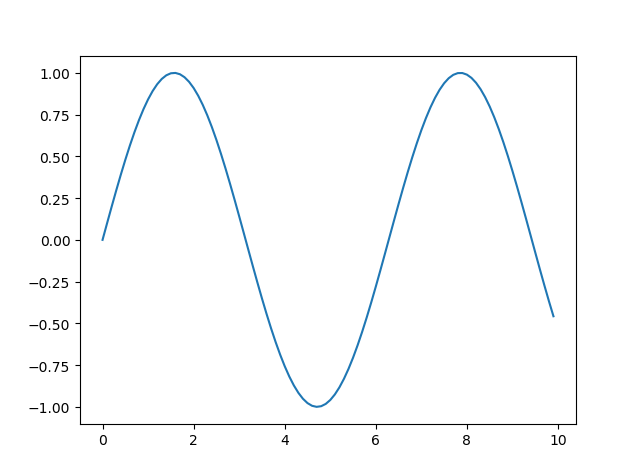
\includegraphics[width = 7cm, height = 5cm]{figure/sinx.png}}\subfigure[~pandas]{
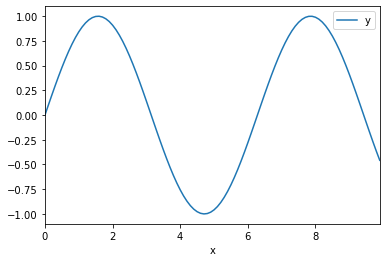
\includegraphics[width = 7cm, height = 5cm]{figure/sinx-pandas.png}}
  \caption{$y=sin(x)$ 的 matplotlib 与 pandas的 画图效果}\label{fig:sinx}

\end{figure}

\vspace{3pt}
\noindent\textbf{3. seaborn 画图的基本用法}
\vspace{3pt}

使用 seaborn 画图时,最基本的图形是线图 lineplot,对于上面的数据,seaborn 画图的代码如下:
\begin{lstlisting}[Language=Python]
import seaborn as sns

x = np.arange(0, 10, 0.1) # 横坐标数据为从0到10之间,步长为0.1的等差数组
y = np.sin(x) # 纵坐标数据为 x 对应的 sin(x) 值

sns.lineplot(x, y)
\end{lstlisting}

显示效果如图 \ref{fig:sinx-sns},如果使用 seaborn 的画图美化,在 seanborn 画图风格前添加一行代码 sns.set(),则使用默认的美化风格:

\begin{lstlisting}[Language=Python]
import seaborn as sns

x = np.arange(0, 10, 0.1) # 横坐标数据为从0到10之间,步长为0.1的等差数组
y = np.sin(x) # 纵坐标数据为 x 对应的 sin(x) 值

sns.set()
sns.lineplot(x, y)
\end{lstlisting}

添加 sns.set() 之后的画图效果如图 \ref{fig:sinx-sns},明显可以看出使用 seaborn 的美化效果之后,图片更好看了。

\begin{figure}[ht]
  \centering
  \subfigure[~不使用 sns.set()]
  {\includegraphics[width = 7cm, height = 5cm]{figure/sinx-sns-a.png}}\subfigure[~使用 sns.set() 美化]{
\includegraphics[width = 7cm, height = 5cm]{figure/sinx-sns-b.png}}
  \caption{seaborn 的 画图效果}\label{fig:sinx-sns}

\end{figure}


\section{三个画图包的高级设置}

利用plot函数,我们可以对图形进行更多精细的设置,官方的详细文档可以参看: \href{https://matplotlib.org/3.1.1/api/\_as\_gen/matplotlib.pyplot.plot.html}{https://matplotlib.org/3.1.1/api/\_as\_gen/matplotlib.pyplot.plot.html}。Plot 函数的基本语法是:


\begin{center}
\begin{tcolorbox}[title = plot 函数的语法]
\textbf{plot([x], y, [fmt], **kwargs)}
\tcblower
\vspace{10pt}

\begin{tcboutputlisting}
\begin{tabular}{>{\bfseries}ll}
  [x] &可选参数,横坐标轴数据\\
  y & 纵坐标轴数据\\

[fmt] &可选参数,字符串,定义图形的基本样式:颜色,点形,线形\\
**kwargs &不定长的关键字参数,用字典形式设置图形的其他属性
\end{tabular}
\end{tcboutputlisting}
\tcbuselistingtext

\end{tcolorbox}
\end{center}

[fmt] 的常用代码(包括颜色代码、点形代码、线形代码),由表 \ref{table:plotParams} 所示。

\begin{table}[ht]
  \centering
  \caption{Plot 函数中的颜色、点形、线性代码}\label{table:plotParams}
  \vspace{5pt}
  \begin{subtable}{.3\linewidth}
    \caption{Plot 函数的颜色代码}
  \begin{tabular}{ll}
    \toprule
    颜色代码 & 颜色\\
    \midrule
    \textquotesingle b\textquotesingle & 蓝色\\
    \textquotesingle r\textquotesingle & 红色\\
    \textquotesingle g\textquotesingle & 绿色 \\
    \textquotesingle k\textquotesingle & 黑色\\
    \textquotesingle w\textquotesingle & 白色\\
    \textquotesingle y\textquotesingle & 黄色 \\
    \bottomrule
  \end{tabular}
\end{subtable}
\begin{subtable}{.3\linewidth}
  \caption{Plot 函数的点形代码}
\begin{tabular}{ll}
  \toprule
  线形代码 & 线形\\
  \midrule
  \textquotesingle o\textquotesingle & 实心圆形\\
  \textquotesingle .\textquotesingle & 点形\\
  \textquotesingle +\textquotesingle & 十字形\\
  \textquotesingle *\textquotesingle & 星号 \\
    \textquotesingle +\textquotesingle & 加号 \\
  \textquotesingle x\textquotesingle & 叉号\\
  \bottomrule
\end{tabular}
\end{subtable}
  \begin{subtable}{.3\linewidth}
    \caption{Plot 函数的线形代码}
  \begin{tabular}{ll}
    \toprule
    线形代码 & 线形\\
    \midrule
    \textquotesingle -\textquotesingle & 实线\\
    \textquotesingle -{}-\textquotesingle & 虚线\\
    \textquotesingle -.\textquotesingle & 折线 \\
    \textquotesingle :\textquotesingle & 点线\\

    &\\
    \bottomrule
  \end{tabular}
\end{subtable}
\end{table}

**kwargs 的常用设置包括线条的粗细 linewidth(或写成 lw),图像标签  label 等。下面一些 plot 函数的代码展示了 [x],[fmt],**Kwargs 的一些可选用法。

\clearpage

\begin{lstlisting}[Language= Python]
>>> plot(x, y)        # 根据横坐标数据 x 与纵坐标数据 y 画图,采用默认的颜色、点形与线性
>>> plot(y)           # 据纵坐标数据 y 画图,横坐标数据默认为从 0 到 N-1,步长为 1 的等差数组
>>> plot(x, y, 'bo')  # 颜色为蓝色('b')、点形为圆('o')
>>> plot(y, 'g-.')     # 颜色为绿色('g'),线形为折线('-.')
>>> plt.plot(x, y, 'yo:', label='y=sin(x)', lw=2) # 颜色为黄色('y'),点形为圆形('o'),线形为虚线(':'),lable 内容为 'y=sin(x)', 线条宽度为 2
\end{lstlisting}


如果我们想自定义坐标轴的标题,坐标轴的刻度,坐标轴刻度的范围,设置图形标题,添加图例时,可以通过设置 pyplot 函数中的 xlable(横坐标轴标题), ylabel(纵坐标轴标题), xticks(横坐标轴刻度),yticks(纵坐标轴刻度),title(图形标题), grid(显示网格),legend(显示图例)等属性来实现。经过自定义设置,对图 \ref{fig:sinx} 的代码进行一下修改,生成图 \ref{fig:sinx2}。


\begin{lstlisting}[Language = Python]
# 导入工具包
import matplotlib.pyplot as plt
import numpy as np

# 这两行代码使得 pyplot 画出的图形中可以显示中文
plt.rcParams['font.sans-serif'] = ['SimHei']
plt.rcParams['axes.unicode_minus'] = False

# 生成数据
x = np.arange(0, 10, 0.5)
y = np.sin(x)

# 生成图形
plt.plot(x, y, 'go:', label='y=sin(x)', linewidth=2) # 颜色绿色,点形圆形,线性虚线,设置图例显示内容,线条宽度为2

plt.ylabel('y') # 横坐标轴的标题
plt.xlabel('x') # 纵坐标轴的标题
plt.xticks(np.arange(0, 11, 1)) # 设置横坐标轴的刻度为 0 到 10 的数组
plt.ylim([-2, 2]) # 设置纵坐标轴范围为 -2 到 2
plt.legend() # 显示图例, 图例中内容由 label 定义
plt.grid() # 显示网格
plt.title('我的第一个 Python 图形') # 图形的标题

# 显示图形
plt.show()

\end{lstlisting}

\begin{figure}[!ht]
  \centering
  \includegraphics[width=\textwidth]{figure/sinx2.png}
  \caption{自定义坐标轴标题、刻度、范围,显示图例、网格与图形标题}\label{fig:sinx2}
\end{figure}


\section{常用图形的绘制}
\subsection{线图}

在统计学中,线图一般用来表示时间序列数据,线图称为趋势图(run chart),因为从线图中可以清晰地看出数据虽时间变化的趋势。 表 \ref{table:GDP} 是我国近10年的 GDP 增长率,以及三大产业在近10年的增长率。


\begin{table}[!ht]
\centering
\renewcommand{\arraystretch}{1.2}
\caption{我国近10年的经济增长率, 数据来源:国家统计局}\label{table:GDP}
\begin{tabular}{|l|l|l|l|l|}
\hline

时间 & GDP增长率 & 第一产业增长率 & 第二产业增长率 & 第三产业增长率 \\ \hline
2009年 & 9.40  & 4.00  & 10.30  & 9.60  \\ \hline
2010年 & 10.60  & 4.30  & 12.70  & 9.70  \\ \hline
2011年 & 9.60  & 4.20  & 10.70  & 9.50  \\ \hline
2012年 & 7.90  & 4.50  & 8.40  & 8.00  \\ \hline
2013年 & 7.80  & 3.80  & 8.00  & 8.30  \\ \hline
2014年 & 7.30  & 4.10  & 7.40  & 7.80  \\ \hline
2015年 & 6.90  & 3.90  & 6.20  & 8.20  \\ \hline
2016年 & 6.70  & 3.30  & 6.30  & 7.70  \\ \hline
2017年 & 6.80  & 4.00  & 5.90  & 7.90  \\ \hline
2018年 & 6.60  & 3.50  & 5.80  & 7.60 \\ \hline
\end{tabular}
\end{table}



在画图时,横坐标轴数据为年份,纵坐标轴数据分别为 GDP 增长率,第一产业增长率,第二产业增长率,第三产业增长率。为了将四个纵坐标轴数据显示在一个图形上,可以用四个 plot 函数进行划线。

\vspace{3pt}
\noindent\textbf{1. matplotlib 画图}
\vspace{3pt}

matplotlib 画图的代码为:

\begin{lstlisting}[Language = Python]
import matplotlib.pyplot as plt

# 这两行代码解决 plt 中文显示的问题
plt.rcParams['font.sans-serif'] = ['SimHei']
plt.rcParams['axes.unicode_minus'] = False

# 输入纵坐标轴数据与横坐标轴数据
gdp_rate = [9.4, 10.6, 9.6, 7.9, 7.8, 7.3, 6.9, 6.7, 6.8, 6.6]
first_industry_rate = [4.0, 4.3, 4.2, 4.50, 3.8, 4.1, 3.9, 3.3, 4.0, 3.5]
second_industry_rate = [10.3, 12.7, 10.7, 8.4, 8.0, 7.4, 6.2, 6.3, 5.9, 5.8]
third_industry_rate = [9.6, 9.7, 9.5, 8.0, 8.3, 7.8, 8.2, 7.7, 7.9, 7.6]
years = [2009, 2010, 2011, 2012, 2013, 2014, 2015, 2016, 2017, 2018]

# 4 个 plot 函数画出 4 条线,线形为折线,每条线对应各自的标签 label
plt.plot(years, gdp_rate, '.-', label='GDP增长率')
plt.plot(years, first_industry_rate, '.-', label='第一产业增长率')
plt.plot(years, second_industry_rate, '.-', label='第二产业增长率')
plt.plot(years, third_industry_rate, '.-', label='第三产业增长率')

plt.xticks(years)  # 设置横坐标刻度为给定的年份
plt.xlabel('年份') # 设置横坐标轴标题
plt.legend() # 显示图例,即每条线对应 label 中的内容
plt.show() # 显示图形
\end{lstlisting}

显示效果如图 \ref{fig:gdp} 所示。

\begin{figure}[!ht]
\centering
  \includegraphics[width=\textwidth]{figure/gdp.png}
  \caption{近十年我国的 GDP 以及各产业增长率}\label{fig:gdp}
\end{figure}

\subsection{散点图}

散点图是数据点在直角坐标系平面上的分布图,在统计学的回归分析与预测中经常用到。用横轴代表变量 $x$,纵轴代表变量 $y$,每组数据 $(x_i, y_i)$ 在坐标系中用一个点表示。
做散点图要用到 pyplot 中的 scatter 函数,该函数的基本语法为\footnote{在 matplotlib 工具包中,0 到 1 之间的浮点数产生相应的 RGB 颜色}:

\begin{center}
\begin{tcolorbox}[title = scatter 函数的语法]
\textbf{scatter(x, y, [s], [c], **kwargs)}
\tcblower
\vspace{10pt}

\begin{tcboutputlisting}
\begin{tabular}{>{\bfseries}ll}
  x &横坐标轴数据\\
  y & 纵坐标轴数据\\

[s] &可选参数,一个数或一个数组,设置每个散点的大小\\

[c] &可选参数,一个数或一个数组,设置每个散点的颜色\\
**kwargs &不定长的关键字参数,用字典形式设置图形的其他属性
\end{tabular}
\end{tcboutputlisting}
\tcbuselistingtext

\end{tcolorbox}
\end{center}

**kwargs 中常设置的是不透明度属性 alpha,其大小为0到1之间的浮点数。假设某个农产品的产量与温度和降雨量的关系如表 \ref{table:scatter} 所示。

\begin{table}[!ht]
\centering
\renewcommand{\arraystretch}{1.2}
\caption{某农产品的产量与温度和降雨量的关系}\label{table:scatter}
\begin{tabular}{|l|l|l|l|}
\hline
产量 & 温度 & 降雨量 \\ \hline
1125 & 6 & 25 \\ \hline
1725 & 8 & 40 \\ \hline
2250 & 10 & 58 \\ \hline
2875 & 13 & 68 \\ \hline
2900 & 14 & 110 \\ \hline
3750 & 16 & 98 \\ \hline
4125 & 21 & 120 \\ \hline

\end{tabular}
\end{table}

作出产量与温度的散点图的 Python 代码与图形如下:
\begin{lstlisting}[Language=Python]
import matplotlib.pyplot as plt
import numpy as np

# 这两行代码解决 plt 中文显示的问题
plt.rcParams['font.sans-serif'] = ['SimHei']
plt.rcParams['axes.unicode_minus'] = False

# 输入产量与温度数据
production = [1125, 1725, 2250, 2875, 2900, 3750, 4125]
tem = [6, 8, 10, 13, 14, 16, 21]

colors = np.random.rand(len(tem))  # 颜色数组
plt.scatter(tem, production, s=200, c=colors)  # 画散点图,大小为 200
plt.xlabel('温度')  # 横坐标轴标题
plt.ylabel('产量')  # 纵坐标轴标题
plt.show()
\end{lstlisting}

\begin{figure}[!ht]
  \centering
  \includegraphics[scale=0.9]{figure/scatter1.png}
  \caption{产量与温度的散点图}
\end{figure}

若将散点大小的数据换为第三个变量的数值,则可以作出反映三个变量关系的气泡图。下面的代码和图形做出了一个气泡图。图 \ref{fig:scatter2} 反映了产量与温度、降雨量的关系:温度数值在横坐标轴,降雨量数值在纵坐标轴,降雨量的大小用气泡的大小表示。

\begin{lstlisting}[Language=Python]
import matplotlib.pyplot as plt
import numpy as np

# 这两行代码解决 plt 中文显示的问题
plt.rcParams['font.sans-serif'] = ['SimHei']
plt.rcParams['axes.unicode_minus'] = False

# 输入产量与温度数据
production = [1125, 1725, 2250, 2875, 2900, 3750, 4125]
tem = [6, 8, 10, 13, 14, 16, 21]
rain = [25, 40, 58, 68, 110, 98, 120]

colors = np.random.rand(len(tem))  # 颜色数组
size = production
plt.scatter(tem, rain, s=size, c=colors, alpha=0.6)  # 画散点图, alpha=0.6 表示不透明度为 0.6
plt.ylim([0, 150])  # 纵坐标轴范围
plt.xlim([0, 30])   # 横坐标轴范围
plt.xlabel('温度')  # 横坐标轴标题
plt.ylabel('降雨量')  # 纵坐标轴标题
plt.show()
\end{lstlisting}

\begin{figure}[!ht]
  \centering
  \includegraphics[scale=0.8]{figure/scatter2.png}
  \caption{产量与温度、降雨量关系的气泡图}\label{fig:scatter2}
\end{figure}

也可以画三维散点图,未完待续...

\clearpage

\subsection{条形图}

条形图(bar chart),也称为柱状图,是一种以长方形的长度为变量的统计图表,长方形的长度与它所对应的变量数值呈一定比例。画条形图要用到 pyplot 中的 bar 函数,该函数的基本语法为:

\begin{center}
\begin{tcolorbox}[title = bar 函数的语法]
\textbf{bar(x, height, [width],  **kwargs)}
\tcblower
\vspace{10pt}

\begin{tcboutputlisting}
\begin{tabular}{>{\bfseries}ll}
  x &数组,每个条形的横坐标\\
  height & 一个数或一个数组,条形的高度\\

[width] &可选参数,一个数或一个数组,条形的宽度,默认为 0.8\\

**kwargs &不定长的关键字参数,用字典形式设置条形图的其他属性
\end{tabular}
\end{tcboutputlisting}
\tcbuselistingtext
\end{tcolorbox}
\end{center}

**kwargs 中常设置的参数包括图形标签 label,颜色标签 color,不透明度 alpha 等。假设某项针对男女大学生购买饮用水爱好的调查结果如下表:

\begin{table}[!ht]
\centering
\caption{男女大学生购买饮用水爱好调查表}
\renewcommand{\arraystretch}{1.2}
\begin{tabular}{|l|l|l|l|}
\hline
买水选择 & 男 & 女 \\ \hline
碳酸饮料 & 6 & 9 \\ \hline
绿茶 & 7 & 4 \\ \hline
矿泉水 & 6 & 4 \\ \hline
果汁 & 1 & 5 \\ \hline
其他 & 2 & 6 \\ \hline
总计 & 22 & 28 \\ \hline
\end{tabular}
\end{table}

画出男生饮用水情况的直方图,代码如下:

\begin{lstlisting}[Language=Python]
import matplotlib.pyplot as plt

# 这两行代码解决 plt 中文显示的问题
plt.rcParams['font.sans-serif'] = ['SimHei']
plt.rcParams['axes.unicode_minus'] = False

waters = ('碳酸饮料', '绿茶', '矿泉水', '果汁', '其他')
buy_number = [6, 7, 6, 1, 2]

plt.bar(waters, buy_number)
plt.title('男性购买饮用水情况的调查结果')

plt.show()
\end{lstlisting}

显示的图形:
\begin{figure}[!ht]
  \centering
  \includegraphics[scale=0.8]{figure/bar1.png}
  \caption{男性购买饮用水条形图}
\end{figure}


若要生成横的条形图,则可以使用 barh 函数,其语法与 bar 函数非常类似。

\begin{center}
\begin{tcolorbox}[title = barh 函数的语法]
\textbf{barh(x, width, [height], **kwargs)}
\tcblower
\vspace{10pt}

\begin{tcboutputlisting}
\begin{tabular}{>{\bfseries}ll}
    y &数组,每个条形的纵坐标\\
    width & 一个数或一个数组,条形的宽度\\

  [height] &可选参数,一个数或一个数组,条形的高度,默认为 0.8\\

**kwargs &不定长的关键字参数,用字典形式设置条形图的其他属性
\end{tabular}
\end{tcboutputlisting}
\tcbuselistingtext
\end{tcolorbox}
\end{center}

对应的代码与图形为:

\begin{lstlisting}[Language=Python]
import matplotlib.pyplot as plt

# 这两行代码解决 plt 中文显示的问题
plt.rcParams['font.sans-serif'] = ['SimHei']
plt.rcParams['axes.unicode_minus'] = False

waters = ('碳酸饮料', '绿茶', '矿泉水', '果汁', '其他')
buy_number = [6, 7, 6, 1, 2]

plt.barh(waters, buy_number)  # 横放条形图函数 barh
plt.title('男性购买饮用水情况的调查结果')

plt.show()
\end{lstlisting}

\begin{figure}[!ht]
  \centering
  \includegraphics[scale=0.9]{figure/bar2.png}
  \caption{男性购买饮用水条形图(条形横放)}\label{fig:bar2}
\end{figure}



若要将男生与女生的调查情况画出两个条形图一块显示,则可以使用 bar 或 barh 函数两次,并调整 bar 或 barh 函数的条形图位置坐标以及相应刻度,使得两组条形图能够并排显示。

\begin{lstlisting}[Language=Python]
import matplotlib.pyplot as plt
import numpy as np

# 这两行代码解决 plt 中文显示的问题
plt.rcParams['font.sans-serif'] = ['SimHei']
plt.rcParams['axes.unicode_minus'] = False

# 输入统计数据
waters = ('碳酸饮料', '绿茶', '矿泉水', '果汁', '其他')
buy_number_male = [6, 7, 6, 1, 2]
buy_number_female = [9, 4, 4, 5, 6]

bar_width = 0.3  # 条形宽度
index_male = np.arange(len(waters))  # 男生条形图的横坐标
index_female = index_male + bar_width  # 女生条形图的横坐标

# 使用两次 bar 函数画出两组条形图
plt.bar(index_male, height=buy_number_male, width=bar_width, color='b', label='男性')
plt.bar(index_female, height=buy_number_female, width=bar_width, color='g', label='女性')

plt.legend()  # 显示图例
plt.xticks(index_male + bar_width/2, waters)  # 让横坐标轴刻度显示 waters 里的饮用水, index_male + bar_width/2 为横坐标轴刻度的位置
plt.ylabel('购买量')  # 纵坐标轴标题
plt.title('购买饮用水情况的调查结果')  # 图形标题

plt.show()
\end{lstlisting}

生成图 \ref{fig:bar3}。
\begin{figure}[!ht]
  \centering
  \includegraphics[scale=0.8]{figure/bar3.png}
  \caption{男女购买饮用水条形图}\label{fig:bar3}
\end{figure}

\clearpage
\subsection{直方图}

直方图(histogram)虽然在样式上类似条形图,但它们的作用不一样。直方图用不同的矩形表示频数,常用来观察一组数据的概率分布。在直角坐标中,用横轴表示数据分组,纵轴表示频数或频率,各组与相应的频数就形成了一个个矩形,即直方图。

画直方图用到 pyplot 中的 hist 函数,它的基本语法为:

\begin{center}
\begin{tcolorbox}[title = hist 函数的语法]
\textbf{[n, bins, patches] = hist(x, [bins], **kwargs)}
\tcblower
\vspace{5pt}

\begin{tcboutputlisting}
\begin{tabular}{>{\bfseries}ll}
  \textbf{输入值:}&\\
    x &数组,需要绘制直方图的数值\\

  [bins] &可选参数,数据的组数,若不指定则 hist 函数默认计算一个组数\\

**kwargs &不定长的关键字参数,用字典形式设置条形图的其他属性\\
&\\
  \textbf{返回值:} &\\
n &一个数组,每组直方图的频数(或概率密度)\\
bins &一个数组,直方图的边界数值\\
patches & 一个对象组,每个对象代表直方图的矩形

\end{tabular}

\tcblower

\end{tcboutputlisting}
\tcbuselistingtext
\end{tcolorbox}
\end{center}

**kwargs 中常用来设置的属性包括直方的边界线颜色 edgecolor,不透明度 alpha 等。需要注意的是,hist 函数的三个返回值一般用来继续对数据进行分析,并不是必须要写或必须要使用的。下面举例说明该函数,例如某个饭店每天接待的顾客数有以下记录值:

\begin{table}[!ht]
\centering
\renewcommand{\arraystretch}{1.2}
\caption{某饭店每天接待的顾客数的记录值}
\begin{tabular}{|l|l|l|l|l|l|l|l|l|l|}
\hline

141 & 159 & 166 & 172 & 177 & 182 & 188 & 196 & 203 & 214 \\ \hline
143 & 160 & 167 & 173 & 177 & 183 & 189 & 196 & 203 & 215 \\ \hline
144 & 160 & 168 & 173 & 178 & 184 & 189 & 196 & 205 & 218 \\ \hline
149 & 161 & 168 & 174 & 178 & 185 & 189 & 196 & 206 & 223 \\ \hline
150 & 161 & 168 & 174 & 178 & 186 & 190 & 196 & 207 & 225 \\ \hline
152 & 162 & 170 & 174 & 179 & 186 & 190 & 197 & 208 & 226 \\ \hline
153 & 163 & 171 & 175 & 179 & 187 & 191 & 197 & 209 & 228 \\ \hline
153 & 163 & 171 & 175 & 179 & 187 & 192 & 198 & 210 & 233 \\ \hline
154 & 164 & 172 & 175 & 180 & 187 & 194 & 198 & 210 & 233 \\ \hline
155 & 165 & 172 & 175 & 180 & 187 & 194 & 200 & 211 & 234 \\ \hline
156 & 165 & 172 & 176 & 181 & 188 & 195 & 201 & 211 & 234 \\ \hline
158 & 165 & 172 & 176 & 182 & 188 & 195 & 202 & 213 & 237 \\ \hline

\end{tabular}
\end{table}

在 Phthon 中编写代码,并画出对应的直方图。

\clearpage
\begin{lstlisting}[Language=Python]
import matplotlib.pyplot as plt

x = [141, 159, 166, 172, 177, 182, 188, 196, 203, 214,
     143, 160, 167, 173, 177, 183, 189, 196, 203, 215,
     144, 160, 168, 173, 178, 184, 189, 196, 205, 218,
     149, 161, 168, 174, 178, 185, 189, 196, 206, 223,
     150, 161, 168, 174, 178, 186, 190, 196, 207, 225,
     152, 162, 170, 174, 179, 186, 190, 197, 208, 226,
     153, 163, 171, 175, 179, 187, 191, 197, 209, 228,
     153, 163, 171, 175, 179, 187, 192, 198, 210, 233,
     154, 164, 172, 175, 180, 187, 194, 198, 210, 233,
     155, 165, 172, 175, 180, 187, 194, 200, 211, 234,
     156, 165, 172, 176, 181, 188, 195, 201, 211, 234,
     158, 165, 172, 176, 182, 188, 195, 202, 213, 237]

plt.hist(x, edgecolor='k', alpha=0.35) # 设置直方边线颜色为黑色,不透明度为 0.35
plt.show()
\end{lstlisting}

\begin{figure}[!ht]
  \centering
  \includegraphics[scale=0.8]{figure/hist.png}
  \caption{每天接待顾客数分布的直方图}\label{fig:hist}
\end{figure}

从图 \ref{fig:hist} 可以看出,每天的顾客数大致符合一个正态分布。

\subsection{饼图}

饼图(pie char)是一个划分为几个扇形的圆形统计图表,一般用于描述频率或百分比之间的相对关系。在饼图中,每个扇区的弧长(以及圆心角和面积)的大小与其所表示的数量呈固定比例。

画饼图一般使用 pyplot 中的 pie 函数,它的基本语法如下:

\begin{center}
\begin{tcolorbox}[title = pie 函数的语法]
\textbf{pie(x, [expode], [labels], [autopic], **kwargs)}
\tcblower
\vspace{10pt}

\begin{tcboutputlisting}
\begin{tabular}{>{\bfseries}ll}
    x &数组,每个扇区的比例\\

    [expode] & 可选参数,数组,每个扇区突出的大小\\

  [labels] &可选参数,字符串数组,每个扇区的标签\\

  [autopct] &可选参数,字符串或函数,每个扇区显示的数字样式\\

**kwargs &不定长的关键字参数,用字典形式设置条形图的其他属性
\end{tabular}
\end{tcboutputlisting}
\tcbuselistingtext
\end{tcolorbox}
\end{center}

**kwargs 中常用来设置的属性包括是否显示扇区的阴影 shadow, 扇区的起始角度 startangle 等。假设有下列调查数据:

\begin{table}[!ht]
\centering
\renewcommand{\arraystretch}{1.2}
\caption{购水类型的调查数据}
\begin{tabular}{|l|l|}
\hline

购水类型 & 人数 \\ \hline
碳酸饮料 & 15 \\ \hline
绿茶 & 11 \\ \hline
矿泉水 & 10 \\ \hline
其他 & 8 \\ \hline
果汁 & 6 \\ \hline

\end{tabular}
\end{table}

饼图的代码与图形:

\begin{lstlisting}[Language=Python]
import matplotlib.pyplot as plt
import numpy as np

# 这两行代码解决 plt 中文显示的问题
plt.rcParams['font.sans-serif'] = ['SimHei']
plt.rcParams['axes.unicode_minus'] = False

labels = ['果汁', '矿泉水', '绿茶', '其他', '碳酸饮料']
x = [6, 10, 11, 8, 15]
explode = [0, 0.1, 0, 0, 0]  # 突出显示第二个扇区

plt.pie(x, explode=explode, labels=labels, autopct='%.2f%%', shadow=True, startangle=90)
plt.legend()  # 显示标签
plt.axis('equal')  # 让图形和坐标轴相等,这样避免饼图为椭圆形
plt.show()
\end{lstlisting}

\begin{figure}[!ht]
  \centering
  \includegraphics[scale=0.7]{figure/pie1.png}
  \caption{调查结果的饼图}\label{fig:pie}
\end{figure}

若在饼图上既要显示比率,又要显示实际调查数字,则可以通过自定义 autopct 函数来实现:
\begin{lstlisting}[Language=Python]
import matplotlib.pyplot as plt
import numpy as np

# 这两行代码解决 plt 中文显示的问题
plt.rcParams['font.sans-serif'] = ['SimHei']
plt.rcParams['axes.unicode_minus'] = False


# 自定义 autopct 函数
def func(pct, allvals):
    absolute = int(round(pct*np.sum(allvals)/100.0))
    return "{:.1f}%\n({:d})".format(pct, absolute)


labels = ['果汁', '矿泉水', '绿茶', '其他', '碳酸饮料']
x = [6, 10, 11, 8, 15]
explode = [0, 0.1, 0, 0, 0]  # 突出显示第二个扇区

plt.pie(x, explode=explode, labels=labels, autopct=lambda pct: func(pct, x),  # 利用 lambda 定义 pct 函数
        shadow=True, startangle=90)
plt.legend()  # 显示标签
plt.axis('equal')  # 让图形和坐标轴相等,这样饼图会更好看
plt.show()
\end{lstlisting}

\begin{figure}[!ht]
  \centering
  \includegraphics[scale=0.7]{figure/pie2.png}
  \caption{调查结果的饼图(同时显示比例与原始数据)}\label{fig:pie}
\end{figure}

\clearpage
\subsection{箱线图}

箱线图(box plot)在学术论文中经常出现,是一种用来显示一组数据分散情况资料的统计图,由数据的最大值、最小值、中位数、两个四分位数,共五个特征绘制而成。


\begin{table}[!ht]
\centering
\renewcommand{\arraystretch}{1.2}
\caption{学生成绩统计表}
\begin{tabular}{|l|l|l|l|l|l|l|l|l|l|l|l|}
\hline
&\multicolumn{11}{c|}{学生编号}  \\\hline
课程名称 & 1 & 2 & 3 & 4 & 5 & 6 & 7 & 8 & 9 & 10 & 11 \\ \hline
英语 & 76 & 90 & 97 & 71 & 70 & 93 & 86 & 83 & 78 & 85 & 81 \\ \hline
西方经济学 & 93 & 81 & 76 & 88 & 66 & 79 & 83 & 92 & 78 & 86 & 78 \\ \hline
市场营销学 & 74 & 87 & 85 & 69 & 90 & 80 & 77 & 84 & 91 & 74 & 70 \\ \hline
财务管理 & 68 & 75 & 70 & 84 & 73 & 60 & 76 & 81 & 88 & 68 & 75 \\ \hline
统计学 & 55 & 91 & 68 & 73 & 84 & 81 & 70 & 69 & 94 & 62 & 71 \\ \hline
\end{tabular}
\end{table}

Python 代码:
\begin{lstlisting}[Language=Python]
import numpy as np
import matplotlib.pyplot as plt

# 这两行代码解决 plt 中文显示的问题
plt.rcParams['font.sans-serif'] = ['SimHei']
plt.rcParams['axes.unicode_minus'] = False

marks = [[76, 90, 97, 71, 70, 93, 86, 83, 78, 85, 81],
         [93, 81, 76, 88, 66, 79, 83, 92, 78, 86, 78],
         [74, 87, 85, 69, 90, 80, 77, 84, 91, 74, 70],
         [68, 75, 70, 84, 73, 60, 76, 81, 88, 68, 75],
         [70, 73, 92, 65, 78, 87, 90, 70, 66, 79, 68],
         [55, 91, 68, 73, 84, 81, 70, 69, 94, 62, 71]]
courses = ('英语', '西方经济学', '市场营销学', '财务管理', '基础会计学', '统计学')

plt.boxplot(marks)
plt.xticks(np.arange(1, 7), courses)
plt.show()
\end{lstlisting}

显示结果:
\begin{figure}[!ht]
  \centering
  \includegraphics[scale=0.8]{figure/box.png}
  \caption{考试成绩的箱线图}\label{fig:box}
\end{figure}

\section{画子图函数 subplot}

%  \chapter{统计数据的度量,概率分布,生成随机数}

Python 中的统计分析工具包 scipy.stats 包括80多个连续型随机分布以及10个离散型随机分布,结合 Numpy,Pandas 工具包,基本能满足统计分析的全部需要。

\section{统计数据的概括性度量}

统计数据的概括性度量主要包括:均值、方差、众数、中位数、偏度、峰度等。

\subsection{最大值、最小值、求和}

\subsection{均值、方差}

一组数据相加后除以数据的个数得到的结果称作均值。一般的均值可以用 numpy 中的 mean 方法求得:

\begin{lstlisting}[Language=Python]
>>> import numpy as np
>>> a = [5, 6, 16, 9]
>>> np.mean(a)
9.0
\end{lstlisting}

numpy 中的 average 方法不仅能求得简单平均数,也可以求出加权平均数。average 里面可以跟一个 weights 参数,里面是一个权数的数组,例如:

\begin{lstlisting}[Language=Python]
>>> np.average(a)
>>> 9.0
>>> np.average(a, weights = [1, 2, 1, 1])
>>> 8.4
\end{lstlisting}


计算方差时,可以利用 numpy 中的 var 函数,默认是总体方差(计算时除以样本数 N),若需要得到样本方差(计算时除以 N - 1),需要跟参数 ddo f= 1,例如

\begin{lstlisting}[Language=Python]
>>> import pnumpy as np
>>> a = [5, 6, 16, 9]
>>> np.var(a) # 计算总体方差
18.5

>>> np.var(a, ddof = 1) # 计算样本方差
24.666666666666668

>>> b = [[4, 5], [6, 7]]
>>> b
[[4, 5], [6, 7]]

>>> np.var(b) # 计算矩阵所有元素的方差
1.25

>>> np.var(b, axis = 0) # 计算矩阵每一列的方差
array([1., 1.])

>>> np.var(b, axis = 1) # 计算矩阵每一行的方差
array([0.25, 0.25])

\end{lstlisting}

计算标准差时,可以利用 numpy 中的 std 函数,使用方法与 var 函数很像,默认是总体标准差,若需要得到样本标准差,需要跟参数 ddof =1,

\begin{lstlisting}[Language=Python]
>>> import pnumpy as np
>>> a = [5, 6, 16, 9]
>>> np.std(a) # 计算总体标准差
4.301162633521313

>>> np.std(a, ddof = 1 ) # 计算样本标准差
4.96655480858378

>>> np.std(b) # 计算矩阵所有元素的标准差
1.118033988749895

>>> np.std(b, axis = 0) # 计算矩阵每一列的标准差
array([1., 1.])

>>> np.std(b, axis = 1) # 计算矩阵每一列的标准差
array([0.5, 0.5])

\end{lstlisting}



对于 pandas 的 DataFrame 类型,也可以用里面的 mean 函数可以求得所有行或所有列的平均数,例如:

\begin{lstlisting}[Language=Python]
>>> import pandas as pd
>>> df = pd.DataFrame(np.array([[85, 68, 90], [82, 63, 88], [84, 90, 78]]), columns=['统计学', '高数', '英语'], index=['张三', '李四', '王五'])
>>> df
统计学  高数  英语
张三   85  68  90
李四   82  63  88
王五   84  90  78

>>> df.mean() # 显示每一列的平均数

统计学    83.666667
高数     73.666667
英语     85.333333
dtype: float64

>>> df.mean(axis = 1) # 显示每一行的平均数
张三    81.000000
李四    77.666667
王五    84.000000
dtype: float64
\end{lstlisting}

若要得到某一行或某一列的平均值,则可以使用 iloc 选取改行或该列数据,后面跟 mean 函数就能得到,例如:

\begin{lstlisting}[Language=Python]
>>> df
    统计学  高数  英语
张三   85  68  90
李四   82  63  88
王五   84  90  78

>>> df.iloc[0, :].mean()  # 得到第 1 行的平均值
81.0

>>> df.iloc[:, 2].mean() # 得到第 3 列的平均值
85.33333333333333

\end{lstlisting}

pandas 中的 var 函数可以得到样本方差(注意不是总体方差),std 函数可以得到样本标准差,若要得到某一行或某一列的方差,则也可用 iloc 选取某行或某列,后面再跟 var 函数或 std 函数即可,例如:

\begin{lstlisting}[Language=Python]
>>> df.var() # 得到每一列的方差
统计学      2.333333
高数     206.333333
英语      41.333333
dtype: float64

>>> df.var(axis = 1) # 得到每一行的方差
张三    133.000000
李四    170.333333
王五     36.000000
dtype: float64

>>> df.std() # 得到每一列的标准差
统计学     1.527525
高数     14.364308
英语      6.429101
dtype: float64

>>> df.std(axis = 1) # 得到每一行的标准差
张三    11.532563
李四    13.051181
王五     6.000000
dtype: float64

>>> df.iloc[0, :].std() # 得到第 1 行的标准差
11.532562594670797

>>> df.iloc[:, 2].std() # 得到第 3 列的标准差
6.429100507328636
\end{lstlisting}

\subsection{中位数、分位数、众数}

使用 numpy 的 median 函数可以得到其中位数,quantile 函数可以得到其分位数,但numpy 包目前还没有计算众数的函数。例如:

\begin{lstlisting}[Language=Python]
>>> a = [8, 19, 34, 9, 18]
>>> np.median(a) # 得到数组 a 的中位数
18.0

>>> np.quantile(a, 0.25) # 得到数组 a 的上四分位数
9.0

>>> np.quantile(a, 0.5) # 得到数组 a 的中位数
18.0

>>> np.quantile(a, 0.75) # 得到数组 a 的下四分位数
19.0
\end{lstlisting}

pandas 可以使用 median,quantile,mode 函数分别计算中位数,分位数与众数。例如:

\begin{lstlisting}[Language=Python]
>>> df = pd.DataFrame(np.array([[85, 68, 90], [82, 63, 88], [84, 90, 88]]), columns=['统计学', '高数', '英语'], index=['张三', '李四', '王五'])
>>> df

    统计学  高数  英语
张三   85  68  90
李四   82  63  88
王五   84  90  88

>>> df.median() # 得到每一列的中位数
统计学    84.0
高数     68.0
英语     88.0
dtype: float64

>>> df.iloc[0, :].median() # 得到第一行的中位数
85.0

>>> df.quantile(0.25, axis = 1) # 得到所有行的上四分位数
张三    76.5
李四    72.5
王五    86.0
Name: 0.25, dtype: float64

>>> df.iloc[2, :].quantile(0.75) # 得到第三行的下四分位数
89.0

>>> df.mode()  # 得到所有列的众数
   统计学  高数    英语
0   82  63  88.0
1   84  68   NaN
2   85  90   NaN

\end{lstlisting}

\subsection{偏度、峰度}

在计算一个样本的偏度或峰度时,对于一般的数组类型,要用到统计分析工具包 scipy,对于 pandas 中的数据类型,可以调用 pandas 自带的计算偏度或峰度的函数。


\begin{lstlisting}[Language=Python]
>>> import scipy.stats as st
>>> a = [89, 23, 45, 18]

>>> st.skew(a) # 计算偏度
0.7565543738808015

>>> st.kurtosis(a) # 计算峰度
-1.0489580648783101
\end{lstlisting}


需要注意的是,pandas 计算峰度时需要至少 4 个数据。
\begin{lstlisting}[Language=Python]
>>> import pandas as pd
>>> import numpy as np
>>> df = pd.DataFrame(np.array([[85, 68, 90], [82, 63, 88], [84, 90, 78]]), columns=['统计学', '高数', '英语'], index=['张三', '李四', '王五'])
>>> df
    统计学  高数  英语
张三   85  68  90
李四   82  63  88
王五   84  90  78

>>> df.iloc[1, :].skew() # 计算第二行的偏度
-1.3294040702410526

>>> df.skew(axis = 0) # 计算所有列的偏度
统计学   -0.935220
高数     1.498959
英语    -1.545393
dtype: float64

>>> df.skew(axis = 1) # 计算所有行的偏度
张三   -1.373033
李四   -1.329404
王五    0.000000
dtype: float64

>>> df1 = pd.DataFrame(np.array([[85, 68, 90, 65], [82, 63, 88, 83], [84, 90, 78, 90], [72, 68, 91, 84]]), columns=['统计学', '高数', '英语', '计算机'], index=['张三', '李四', '王五', '马六'])
>>> df1
    统计学  高数  英语  计算机
张三   85  68  90   65
李四   82  63  88   83
王五   84  90  78   90
马六   72  68  91   84

>>> df1.kurt(axis = 0) # 计算 df1 所有列的偏度
统计学    3.090874
高数     3.365664
英语     3.090874
计算机    2.769386
dtype: float64

>>> df1.iloc[:, 2].kurt() #计算 df1 第 3 列的偏度
3.090874188966101
\end{lstlisting}

\section{概率密度、累计分布、逆函数}

计算概率分布的相关参数时,一般使用 scipy 包,常用的函数包括以下几个:

\begin{itemize}
  \item pdf:连续随机分布的概率密度函数
  \item pmf:离散随机分布的概率密度函数
  \item cdf:累计分布函数
  \item ppf:百分位函数(累计分布函数的逆函数)
  \item isf: 生存函数的逆函数(1 - cdf 的逆函数)
\end{itemize}

函数里面不仅能跟一个数据,还能跟一个数组。下面用正态分布举例说明:

\begin{lstlisting}[Language=Python]
>>> import scipy.stats as st

>>> st.norm.cdf(0) # 标准正态分布在 0 处的累计分布概率值
0.5

>>> st.norm.cdf([-1, 0, 1])# 标准正态分布分别在 -1, 0, 1 处的累计分布概率值
array([0.15865525, 0.5, 0.84134475])

>>> st.norm.pdf(0) # 标准正态分布在 0 处的概率密度值
0.3989422804014327

>>> st.norm.ppf(0.975)# 标准正态分布在 0.975 处的逆函数值
1.959963984540054

>>> st.norm.lsf(0.975)# 标准正态分布在 0.025 处的生存函数的逆函数值
1.959963984540054
\end{lstlisting}

对于非标准正态分布,通过更改参数 loc 与 scale 来改变均值与标准差:

\begin{lstlisting}[Language=Python]
>>> st.norm.cdf(0, loc=2, scale=1) # 均值为 2,标准差为 1 的正态分布在 0 处的累计分布概率值
0.022750131948179195
\end{lstlisting}

对于其他随机分布,可能更改的参数不一样,具体需要查官方文档。下面我们举一些常用分布的例子:

\begin{lstlisting}[Language=Python]
>>> st.binom.pmf(4, n=100, p=0.05) # 参数值 n=100, p=0.05 的二项分布在 4 处的概率密度值
0.17814264156968956

>>> st.geom.pmf(4, p=0.05) # 参数值 p=0.05 的几何分布在 4 处的概率密度值
0.04286875

>>> st.poisson.pmf(2, mu=3) # 参数值 mu=3 的泊松分布在 2 处的概率密度值
0.22404180765538775

>>> st.chi2.ppf(0.95, df=10) # 自由度为 10 的卡方分布在 0.95 处的逆函数值
18.307038053275146

>>> st.t.ppf(0.975, df=10) # 自由度为 10 的 t 分布在 0.975 处的逆函数值
2.2281388519649385

>>> st.f.ppf(0.95, dfn=2, dfd=12) # 自由度为 2, 12 的 F 分布在 0.95 处的逆函数值
3.8852938346523933
\end{lstlisting}


\section{标准化数据}

\section{生成随机数}

\subsection{用 Numpy 生成随机数}
在 python 中生成随机数有多种方法,首先可以用 Numpy 包的 random 函数生成随机数。例如,生成2 行 2 列, [1, 10] 内的均匀分布随机数:

\begin{lstlisting}[Language=Python]
>>> import numpy as np
>>> np.random.uniform(low=1, high=10, size=[2, 2])
array([[2.42454708, 5.54082358],
       [3.19289445, 3.4544002 ]])
\end{lstlisting}

生成一个正态分布的 2 行 2 列随机数,均值为 5, 标准差为 1:

\begin{lstlisting}[Language=Python]
>>> np.random.normal(loc=5, scale=1, size=[2,2])
array([[4.37643895, 6.00357154],
       [4.76599409, 4.64680265]])
\end{lstlisting}

生成一个泊松分布的 2 行 2 列随机数,均值为 5:

\begin{lstlisting}[Language=Python]
>>> np.random.poisson(mu=5, size=[2,2])
array([[3, 6],
       [7, 5]])
\end{lstlisting}


生成一个指数分布的 2 行 2 列随机数,均值为 5:

\begin{lstlisting}[Language=Python]
>>> np.random.exponential(scale=5, size=[2,2])
array([[3.14056456, 2.63627222],
       [5.44436781, 2.6088458 ]])
\end{lstlisting}

\subsection{用 Scipy 生成随机数}
另外一种生成随机数的方法是用 scipy 包不同分布函数自带的 rvs 生成随机数,例如,生成一个正态分布的 2 行 2 列随机数,均值为 5, 标准差为 1:

\begin{lstlisting}[Language=Python]
>>> import scipy.stats as st
>>> st.norm.rvs(loc=5, scale=1, size=[2,2])
array([[3.96964463, 4.14137383],
       [6.36342893, 3.99992325]])
\end{lstlisting}

生成一个指数分布的 2 行 2 列随机数,均值为 5:

\begin{lstlisting}[Language=Python]
>>> st.poisson.rvs(mu=5, size=[2,2])
array([[5, 7],
       [3, 9]])
\end{lstlisting}

\section{z 检验,t 检验, $\chi^2$ 检验}

 Python 中的假设检验一般用到 scipy 或 statsmodels 包,需要注意的是,这两个包里面各种检验的置信度都是 0.05。

\subsection{z 检验}

 对于大样本数据(样本量 $\geq$ 30),或者即使是小样本,但是知道其服从正态分布,并且知道总体分布的方差时,需要用 z 检验。在 python 中,由于 scipy 包没有 z 检验,我们只能用 statsmodels 包中的 ztest 函数。ztest 函数的一般用法在下页显示。

 \begin{table}[ht]
 \centering
 \caption{样本数据1} \label{tab:ztest}
 \begin{tabular}{|l|l|l|l|l|l|l|l|l|l|l|l|}
 \hline

 23 & 36 & 42 & 34 & 39 & 34 & 35 & 42 & 53 & 28 & 49 & 39 \\ \hline
 46 & 45 & 39 & 38 & 45 & 27 & 43 & 54 & 36 & 34 & 48 & 36 \\ \hline
 47 & 44 & 48 & 45 & 44 & 33 & 24 & 40 & 50 & 32 & 39 & 31 \\ \hline

 \end{tabular}
 \end{table}

 对于表格 \ref{tab:ztest} 的样本数据,检测其均值是否为 39, 该问题显然是一个双侧检验,由于样本个数大于 30,则使用 z 检验,python 代码如下:

 \begin{lstlisting}[Language=Python]
 >>> import statsmodels.stats.weightstats as sw
 >>> arr=[23,36,42,34,39,34,35,42,53,28,49,39,
 ... 46,45,39,38,45,27,43,54,36,34,48,36,
 ... 47,44,48,45,44,33,24,40,50,32,39,31]
 >>> sw.ztest(arr, value=39)
 (0.3859224924939799, 0.6995540720244979)
 \end{lstlisting}

 \begin{center}
 \begin{tcolorbox}[title = ztest 函数的语法]
 \textbf{ztest(x1, x2=None, value=0, alternative=`two-sided')}
 \tcblower
 \vspace{2pt}
 \begin{tcboutputlisting}
 \begin{tabular}{>{\bfseries}ll}
   输入参数:&\\
   x1 &数组,第一个样本的数据值\\
   x2 & 数组,第二个样本的数据值,默认没有值\\
   \specialrule{0em}{2pt}{2pt}
\multirow{2}*{value} &浮点型数值,若是单样本,则 value 是样本假设的均值,\\
&若是双样本,则 value是两个样本均值的差值\\
\specialrule{0em}{2pt}{2pt}
 \multirow{3}*{alternative}&字符串,备选假设 H1,默认为 two-sided',表示双侧检验,\\
 & 若为 `larger',备选假设 H1 大于 value 值\\
 & 若为 `smaller',备选假设 H1 小于 value 值\\
\specialrule{0em}{2pt}{2pt}
 返回值:&\\
 tstats & 统计量值\\
 pvalue & p 值
 \end{tabular}
 \end{tcboutputlisting}
 \tcbuselistingtext

  \end{tcolorbox}
  \end{center}


从 ztest 的运行结果可以看出,统计量值为 0.385,而 p 值是 0.699,在置信度 $\alpha=0.05$ 时,由于 p 值大于 $\alpha$,接受原假设,认为该样本的均值是 39。

若要检测该样本均值是否大于 39,即原假设 H0:$\mu>39$,备选假设为:$\mu\leq 39$,则我们需要在代码中增加一个参数 alternative=``smaller”:

\begin{lstlisting}[Language=Python]
>>> sw.ztest(arr, value=39, alternative="smaller")
(0.3859224924939799, 0.650222963987751)
\end{lstlisting}

检测结果的 p 值为 0.650,大于置信度 0.05,则接受原假设,认为样本均值大于39。假设另外一个样本 2 的数据:

\begin{table}[ht]
\centering
\caption{样本数据2}
\begin{tabular}{|l|l|l|l|l|l|l|l|l|l|}
\hline
41  & 34  & 36  & 32  & 32  & 35  & 33  & 31  & 35  & 34  \\ \hline
37  & 34  & 31  & 36  & 37  & 34  & 33  & 37  & 33  & 38  \\ \hline
38  & 37  & 34  & 36  & 36  & 31  & 33  & 36  & 37  & 35  \\ \hline
33  & 34  & 33  & 35  & 34  & 34  & 34  & 35  & 35  & 34 \\ \hline
\end{tabular}
\end{table}

检测两个样本的均值是否相等,因为两个样本都是大样本,使用 z 检验, python 代码如下:
\begin{lstlisting}[Language=Python]
>>> arr2 = [41, 34, 36, 32, 32, 35, 33, 31, 35, 34,
... 37, 34, 31, 36, 37, 34, 33, 37, 33, 38,
... 38, 37, 34, 36, 36, 31, 33, 36, 37, 35,
... 33, 34, 33, 35, 34, 34, 34, 35, 35, 34]
>>> sw.ztest(arr, arr2, value=0)
(3.775645601380307, 0.0001595937672736755)
\end{lstlisting}

从 ztest 的检验结果可以看出,p 值小于 0.05, 则拒绝原假设,认为两个样本的均值不相等。

\subsection{t 检验}
小样本(样本量小于30个),一般用 t 检验。对于 t 检验,可以根据样本特点,用 scipy 包中的 ttest\_1sample(单样本 t检验函数),ttest\_ind(两个独立样本的 t 检验),ttest\_rel (两个匹配样本的 t 检验)。但这些函数得到都是双侧 t 检验的 p 值。如果是单侧检验,我们还要进行一些换算,得到单侧检验的 p 值。

ttest\_1sample 函数的语法为:

\begin{center}
\begin{tcolorbox}[title = ttest\_1sample 函数的语法]
\textbf{ttest\_1samp(a, popmean)}
\tcblower
\vspace{2pt}
\begin{tcboutputlisting}
\begin{tabular}{>{\bfseries}ll}
  输入参数:&\\
  a &数组,样本的数据值\\
  popmean & 原假设 $H_0$ 中样本的期望值\\
\specialrule{0em}{2pt}{2pt}
返回值:&\\
statistic & 统计量值\\
pvalue & 双侧检验的 p 值
\end{tabular}
\end{tcboutputlisting}
\tcbuselistingtext
\end{tcolorbox}
\end{center}

下面是一个样本的数据:
\begin{equation}
  99.3\quad 98.7\quad 100.5\quad 101.2\quad 98.3\quad 99.7\quad 99.5\quad 102.1\quad 100.5\nonumber
\end{equation}

检测样本均值是否等于100,对其进行双侧 t 检验的语法为:

\begin{lstlisting}[Language=Python]
>>> import scipy.stats as st
>>> a = [99.3, 98.7, 100.5, 101.2, 98.3, 99.7, 99.5, 102.1, 100.5]
>>> st.ttest_1samp(a, 100)
Ttest_1sampResult(statistic=-0.054996133220328265, pvalue=0.9574902045208937)
\end{lstlisting}

从结果可以看出,双侧检验的 p 值为 0.95, 大于置信度 0.05,因此接受原假设,认为样本的均值是100。若是单侧检验中的左侧检验,则 p 值为 $0.957/2=0.4785$,若是右侧检验,则 p 值为 $1-0.957/2=0.5215$。

假设有另外一个样本的数据:
\begin{equation}
91.1\quad 93.7\quad 93.6\quad 96.1\quad 94.3\quad
       92.2\quad 94.0\quad 95.7\quad 97.1 \nonumber
\end{equation}

若两个样本相互独立,检测两个样本的均值是否相等,使用 ttest\_ind 函数。

\begin{center}
\begin{tcolorbox}[title = ttest\_ind 函数的语法]
\textbf{ttest\_ind(a, b, axis=0, equal\_var=True) }
\tcblower
\vspace{2pt}
\begin{tcboutputlisting}
\begin{tabular}{>{\bfseries}ll}
  输入参数:&\\
  a &数组,样本1的数据值\\
  b &数组,样本2的数据值\\
  axis & 一般为 0\\
  \multirow{2}{*}{equal\_var} & 若为 true,表示两个样本由相同的方差\\
  &若为 false,表示两个样本的方差不同,使用合并方差\\
\specialrule{0em}{2pt}{2pt}
返回值:&\\
statistic & 统计量值\\
pvalue & 双侧检验的 p 值
\end{tabular}
\end{tcboutputlisting}
\tcbuselistingtext
\end{tcolorbox}
\end{center}

假设两个样本的方差不同,则独立双样本的 t 检验 python 代码为:

\begin{lstlisting}[Language=Python]
>>> import scipy.stats as st
>>> a = [99.3, 98.7, 100.5, 101.2, 98.3, 99.7, 99.5, 102.1, 100.5]
>>> b = [91.1, 93.7, 93.6, 96.1, 94.3, 92.2, 94.0, 95.7, 97.1]
>>> st.ttest_ind(a, b, equal_var = False)
Ttest_indResult(statistic=7.723221821038956, pvalue=2.4331092243754622e-06)
\end{lstlisting}

从上面结果可以看出,p 值小于置信度 0.05,拒绝原假设,认为两个两个样本的均值不同。

若两个样本是匹配样本,使用函数 ttest\_rel,它的语法更简单,只需在函数里输入两个样本的数组即可。假设上面两个样本为匹配样本,python 代码为:

\begin{lstlisting}[Language=Python]
>>> import scipy.stats as st
>>> a = [99.3, 98.7, 100.5, 101.2, 98.3, 99.7, 99.5, 102.1, 100.5]
>>> b = [91.1, 93.7, 93.6, 96.1, 94.3, 92.2, 94.0, 95.7, 97.1]
>>> st.ttest_rel(a, b)
Ttest_relResult(statistic=10.845107419335658, pvalue=4.617509769582176e-06)
\end{lstlisting}

结果显示,p 值小于置信度 0.05,拒绝原假设,认为这两个匹配样本的均值不同。

\chapter{方差分析}

方差分析用于研究一个或多个分类型自变量与一个数值型因变量之间的关系,即检测多个总体的均值是否相等,一般要使用 F 检验。

\section{单因素方差分析}

\subsection{使用 scipy 的 f\_oneway 函数}
对于单因素方差分析, 其中一个方法是使用 scipy 包提供了 f\_oneway 函数。

例如了调查了三个行业的投诉次数,希望分析行业类别对投诉次数是否有影响。各样本的数据如下所示:
\begin{align}
  \text{零售业:}&57~~ 66~~ 49~~ 40~~ 34~~ 53~~ 44\nonumber\\
  \text{旅游业:}&68~~ 39~~ 29~~ 45~~ 56~~ 51\nonumber\\
  \text{制造业:}&44~~ 51~~ 65~~ 77~~/+ 58\nonumber
\end{align}

使用 f\_oneway 函数做单因素方差分析 F 检验的 python 代码为:

\begin{lstlisting}[Language=Python]
>>> import scipy.stats as st
>>> a = [57, 66, 49, 40, 34, 53, 44]
>>> b = [68, 39, 29, 45, 56, 51]
>>> c = [44, 51, 65, 77, 58]
>>> st.f_oneway(a, b, c)
F_onewayResult(statistic=1.3141307534447377, pvalue=0.29792936408490506)
\end{lstlisting}

从结果可以看出, p 值大于 0.05,则可以认为在 95\% 的置信度内接受愿家人,认为行业类别对投诉次数没有影响。

\subsection{使用 statsmodels 的 anova\_lm 函数}
若想要更详细的方差分析结果,或者多个因素的方差分析,就要使用 statsmodels 包了,statsmodels 包常常结合 pandas 包一起使用。例如,下面的数据存储在 complainNumber.xlsx 的 excel 文件中,

\begin{figure}[ht]
  \centering
  \includegraphics{figure/chapter3/complain.png}
\end{figure}

在做方差分析时,我们需要转化成因变量对应自变量的形式,即将上面的数据转化为下面的形式:

\begin{figure}[ht]
  \centering
  \includegraphics{figure/chapter3/complain2.png}
\end{figure}

通过 excel 转化好形式后,我们再导入到 pandas 数据库中。

\begin{lstlisting}[Language=Python]
>>> df = pd.read_excel(r'D:\Users\chen_\git\Statistics-book\datas\complainNumber.xlsx')
>>> df.head()
    行业  投诉次数
0  零售业    57
1  零售业    66
2  零售业    49
3  零售业    40
4  零售业    34
\end{lstlisting}

对于数据 df,我们首先将它放进 statsmodels 中的 OLS 模型里。OLS (ordinary least squares) 表示普通最小二乘模型,在统计分析中经常使用。该模型的建模模仿了 R 语言, 使用 pasty 语言的语法描述统计学公式。 python 代码如下:

\begin{lstlisting}[Language=Python]
>>> import statsmodels.formula.api as sm
>>> model = sm.ols(formula = '投诉次数 ~ C(行业)', data = df).fit()
\end{lstlisting}

其中,formula = `投诉次数 ~ C(行业)' 表示了单因素方差分析的统计学公式, \textasciitilde 左边的投诉次数为因变量,\textasciitilde 右边表示自变量,C 是 category 的缩写,表示行业是分类变量。

建立统计学模型后,再使用 anova\_lm 函数进行方差分析:

\begin{lstlisting}[Language=Python]
>>> from statsmodels.stats.anova import anova_lm
>>> model = sm.ols(formula = '投诉次数 ~ C(行业)', data = df).fit()
>>> result = anova_lm(model)
>>> print(result)
            df       sum_sq     mean_sq         F    PR(>F)
C(行业)      2.0   398.444444  199.222222  1.314131  0.297929
Residual  15.0  2274.000000  151.600000       NaN       NaN

\end{lstlisting}

上面的结果与 scipy 的 f\_oneway 函数的分析结果一致。

\section{双因素方差分析}

对于双因素方差分析,可以分为有交互作用的双因素方差分析和没有交互作用的双因素方差分析,假如有下面的数据,表示不同地区不同品牌的销量,由于是一一对应的数据,这个数据表是没有交互作用的双因素方差分析。


\begin{figure}[ht]
  \centering
  \includegraphics[scale=0.8]{figure/chapter3/twoFactor.png}
\end{figure}

我们首先将其转化为因变量对应自变量的形式:

\begin{figure}[ht]
  \centering
  \includegraphics[scale=0.8]{figure/chapter3/twoFactor2.png}
\end{figure}

用 pandas 读取数据:

\begin{lstlisting}[Language=Python]
>>> df = pd.read_excel(r'D:\Users\chen_\git\Statistics-book\datas\twoFactorANOVA.xlsx')
>>> df.head()
    地区   品牌   销量
0  地区1  品牌1  365
1  地区1  品牌2  345
2  地区1  品牌3  358
3  地区1  品牌4  288
4  地区2  品牌1  350
\end{lstlisting}

构建 OLS 模型:

\begin{lstlisting}[Language=Python]
>>> model = sm.ols(formula = '销量 ~ C(地区) + C(品牌)', data = df).fit()
\end{lstlisting}

formula = `销量 ~ C(地区) + C(品牌)' 表示了无交互作用的双因素方差分析的统计模型。调用 anova\_lm 函数进行方差分析:

\begin{lstlisting}[Language=Python]
>>> result = anova_lm(model)
>>> print(result)
            df    sum_sq      mean_sq          F    PR(>F)
C(地区)      4.0   2011.70   502.925000   2.100846  0.143665
C(品牌)      3.0  13004.55  4334.850000  18.107773  0.000095
Residual  12.0   2872.70   239.391667        NaN       NaN
\end{lstlisting}

从上面结果可以看出, 地区的 p 值大于 0.05,说明地区对销量没有影响;而品牌的 p 值小于 0.05,说明品牌因素对销量有影响。

若对于同样的地区和品牌,有多个数据,则可能存在交互因素,例如下面的数据可能存在交互作用:

\begin{figure}[ht]
  \centering
  \includegraphics[scale=0.8]{figure/chapter3/twoFactor3.png}
\end{figure}


在构建统计模型时,需要改一下表达式:

\begin{lstlisting}[Language=Python]
>>> model = sm.ols(formula = '销量 ~ C(地区) + C(品牌) + C(地区):C(品牌)', data = df).fit()
\end{lstlisting}

调用 anova\_lm 函数生成结果:

\begin{lstlisting}[Language=Python]
>>> result = anova_lm(model)
>>> print(result)
               df        sum_sq      mean_sq         F    PR(>F)
C(地区)         4.0   2625.375000   656.343750  0.310603  0.858125
C(品牌)         3.0  16654.166667  5551.388889  2.627099  0.186915
C(地区):C(品牌)  12.0   9516.458333   793.038194  0.375292  0.915657
Residual      4.0   8452.500000  2113.125000       NaN       NaN
\end{lstlisting}

从 p 值可以看出,两个因素以及他们的交互作用对销量都没有影响。


\section{多元方差分析}

% \chapter{回归分析}

\section{线性回归}

假如有下列 excel 表格的数据:

\begin{figure}[ht]
  \centering
  \includegraphics{figure/linear_regression.png}
\end{figure}

该文件以 lienar\_regression.xlsx 存到电脑上,我们首先用 pandas 包读取该 excel 数据,

\begin{lstlisting}[Language=Python]
>>> import pandas as pd
>>> datas = pd.read_excel(r'D:\Users\chen_\git\Statistics-book\datas\linear_regression.xlsx') # 读取 excel 数据,引号里面是 excel 文件在电脑的存储位置
>>> datas.head() # 显示 excel 数据文件的前 5 行数据
   分行\n编号  不良贷款(亿元)  各项贷款余额(亿元)  本年累计应收贷款(亿元)  贷款项目个数(个)  本年固定资产投资额(亿元)
0       1       0.9        67.3           6.8          5           51.9
1       2       1.1       111.3          19.8         16           90.9
2       3       4.8       173.0           7.7         17           73.7
3       4       3.2        80.8           7.2         10           14.5
4       5       7.8       199.7          16.5         19           63.2

\end{lstlisting}

\subsection{线性回归}

使用 python 做线性回归分析有好几种方式,常用的分别是 scipy 包(只能做一元线性回归),statsmodels 包,以及 sklearn 包。但是,\textcolor{red}{这些包目前都不能处理共线性,即自动剔除部分共线性的变量},这需要自己去编写相应函数。

\subsubsection{使用 scipy 包}

scipy.stats 中的 linregress 函数可以做一元线性回归。假如因变量为 “不良贷款”,自变量为 “各项贷款余额”,全部 python 代码如下:

\begin{lstlisting}[Language=Python]
import scipy.stats as st
import pandas as pd

datas = pd.read_excel(r'D:\Users\chen_\git\Statistics-book\datas\linear_regression.xlsx') # 读取 excel 数据,引号里面是 excel 文件的位置
y = datas.iloc[:, 1] # 因变量为第 2 列数据
x = datas.iloc[:, 2] # 自变量为第 3 列数据

# 线性拟合,可以返回斜率,截距,r 值,p 值,标准误差
slope, intercept, r_value, p_value, std_err = st.linregress(x, y)

print(slope)# 输出斜率
print(intercept) # 输出截距
print(r_value**2) # 输出 R^2
\end{lstlisting}


scipy 中的回归分析比较简单,目前只能做一元线性回归,也不能用来做预测。

\subsubsection{使用 statsmodel 包}

使用 statsmodel 包中的 OLS (普通最小二乘法)函数,可以构建统计模型,并进行线性拟合。假如因变量为 “不良贷款”,自变量为 “各项贷款余额”,则构建最小二乘的模型以及回归分析的代码如下:

\begin{lstlisting}[Language=Python]
>>> import statsmodels.api as sm
>>> y = datas.iloc[:, 1] # 因变量为第 2 列数据
>>> x = datas.iloc[:, 2] # 自变量为第 3 列数据
>>> x = sm.add_constant(x) # 若模型中有截距,必须有这一步
>>> model = sm.OLS(y, x).fit() # 构建最小二乘模型并拟合
>>> print(model.summary()) # 输出回归结果
\end{lstlisting}

回归结果如下图所示:

\begin{figure}[ht]
  \centering
  \includegraphics[scale=0.8]{figure/linearRegressionResult.png}
\end{figure}

若要画出实际数据与预测图形,可以加上下面代码:

\begin{lstlisting}[Language=Python]
# 画图
# 这两行代码在画图时添加中文必须用
>>> plt.rcParams['font.sans-serif'] = ['SimHei']
>>> plt.rcParams['axes.unicode_minus'] = False

>>> predicts = model.predict() # 模型的预测值
>>> x = datas.iloc[:, 2] # 自变量为第 3 列数据
>>> plt.scatter(x, y, label='实际值') # 散点图
>>> plt.plot(x, predicts, color = 'red', label='预测值')
>>> plt.legend() # 显示图例,即每条线对应 label 中的内容
>>> plt.show() # 显示图形
\end{lstlisting}

图形:

\begin{figure}[ht]
  \centering
  \includegraphics[scale=0.5]{figure/lineRegression1.png}
\end{figure}

全部 python 代码如下:

\begin{lstlisting}[Language=Python]
import pandas as pd
import statsmodels.api as sm
import matplotlib.pyplot as plt

datas = pd.read_excel(r'D:\Users\chen_\git\Statistics-book\datas\linear_regression.xlsx') # 读取 excel 数据,引号里面是 excel 文件的位置
y = datas.iloc[:, 1] # 因变量为第 2 列数据
x = datas.iloc[:, 2] # 自变量为第 3 列数据
x = sm.add_constant(x) # 若模型中有截距,必须有这一步
model = sm.OLS(y, x).fit() # 构建最小二乘模型并拟合
print(model.summary()) # 输出回归结果

# 画图
# 这两行代码在画图时添加中文必须用
plt.rcParams['font.sans-serif'] = ['SimHei']
plt.rcParams['axes.unicode_minus'] = False

predicts = model.predict() # 模型的预测值
x = datas.iloc[:, 2] # 自变量为第 3 列数据
plt.scatter(x, y, label='实际值') # 散点图
plt.plot(x, predicts, color = 'red', label='预测值')
plt.legend() # 显示图例,即每条线对应 label 中的内容
plt.show() # 显示图形
\end{lstlisting}

注意:若导入包时使用命令 import statsmodels.formula.api as sm, 则在回归分析时不用添加截距 add\_constant,但是必须使用统计语言给出模型信息,代码如下:

\begin{lstlisting}[Language=Python]
import pandas as pd
import statsmodels.formula.api as sm
import matplotlib.pyplot as plt

datas = pd.read_excel(r'D:\Users\chen_\git\Statistics-book\datas\linear_regression.xlsx') # 读取 excel 数据,引号里面是 excel 文件的位置
model = sm.ols('不良贷款~各项贷款余额', datas).fit() # 构建最小二乘模型并拟合,
                               #此时不用单独输入 x,y了,而是将自变量与因变量用统计语言公式表示,将全部数据导入
print(model.summary()) # 输出回归结果


# 画图
# 这两行代码在画图时添加中文必须用
plt.rcParams['font.sans-serif'] = ['SimHei']
plt.rcParams['axes.unicode_minus'] = False

predicts = model.predict() # 模型的预测值
y = datas.iloc[:, 1] # 因变量为第 2 列数据
x = datas.iloc[:, 2] # 自变量为第 3 列数据
plt.scatter(x, y, label='实际值')
plt.plot(x, predicts, color = 'red', label='预测值')
plt.legend() # 显示图例,即每条线对应 label 中的内容
plt.show() # 显示图形
\end{lstlisting}

在多元回归中,只需把自变量改为多列数据即可,假如不良贷款为因变量,从第3列到第6列都是因变量,则使用 statsmodels 包的全部 python 代码如下:

\begin{lstlisting}[Language=Python]
import pandas as pd
import statsmodels.api as sm
import matplotlib.pyplot as plt

datas = pd.read_excel(r'D:\Users\chen_\git\Statistics-book\datas\linear_regression.xlsx') # 读取 excel 数据,引号里面是 excel 文件的位置
y = datas.iloc[:, 1] # 因变量为第 2 列数据
x = datas.iloc[:, 2:6] # 自变量为第 3 列到第 6 列数据
x = sm.add_constant(x) # 若模型中有截距,必须有这一步
model = sm.OLS(y, x).fit() # 构建最小二乘模型并拟合
print(model.summary()) # 输出回归结果
\end{lstlisting}

统计结果图如下:

\begin{figure}[ht]
  \centering
  \includegraphics[scale=0.8]{figure/linearRegressionResult2.png}
\end{figure}




\subsubsection{使用 sklearn 包}

sklearn 包机器学习中常见的 python 包,可以用来做统计分析时,但它并不能像 statsmodels 那样生成非常详细的统计分析结果。一元回归时,自变量与因变量都需要处理下,对于上面同样的例子:

\begin{lstlisting}[Language=Python]
import pandas as pd
import matplotlib.pyplot as plt
import numpy as np
from sklearn.linear_model import LinearRegression

datas = pd.read_excel(r'D:\Users\chen_\git\Statistics-book\datas\linear_regression.xlsx') # 读取 excel 数据,引号里面是 excel 文件的位置
y = datas.iloc[:, 1] # 因变量为第 2 列数据
x = datas.iloc[:, 2] # 自变量为第 3 列数据

# 将 x,y 分别增加一个轴,以满足 sklearn 中回归模型认可的数据
x = x[:, np.newaxis]
y = y[:, np.newaxis]

model = LinearRegression() # 构建线性模型
model.fit(x, y) # 自变量在前,因变量在后
predicts = model.predict(x) # 预测值
R2 = model.score(x, y) # 拟合程度 R2
print('R2 = %.2f' % R2) # 输出 R2
coef = model.coef_ # 斜率
intercept = model.intercept_ # 截距
print(model.coef_, model.intercept_) # 输出斜率和截距

# 画图
plt.rcParams['font.sans-serif'] = ['SimHei']
plt.rcParams['axes.unicode_minus'] = False

y = datas.iloc[:, 1] # 因变量为第 2 列数据
x = datas.iloc[:, 2] # 自变量为第 3 列数据
plt.scatter(x, y, label='实际值') # 散点图
plt.plot(x, predicts, color = 'red', label='预测值')
plt.legend() # 显示图例,即每条线对应 label 中的内容
plt.show() # 显示图形
\end{lstlisting}


用 sklearn 做多元回归时,全部代码如下:
\begin{lstlisting}[Language=Python]
import pandas as pd
import matplotlib.pyplot as plt
import numpy as np
from sklearn.linear_model import LinearRegression

datas = pd.read_excel(r'D:\Users\chen_\git\Statistics-book\datas\linear_regression.xlsx') # 读取 excel 数据,引号里面是 excel 文件的位置
y = datas.iloc[:, 1] # 因变量为第 2 列数据
x = datas.iloc[:, 2:6] # 自变量为第 3 列到第 6 列数据

# 将 y 分别增加一个轴,以满足 sklearn 中回归模型认可的数据
# 此时由于 x 是多元变量,则不用添加新的轴了
y = y[:, np.newaxis]

model = LinearRegression() # 构建线性模型
model.fit(x, y) # 自变量在前,因变量在后
predicts = model.predict(x) # 预测值
R2 = model.score(x, y) # 拟合程度 R2
print('R2 = %.3f' % R2) # 输出 R2
coef = model.coef_ # 斜率
intercept = model.intercept_ # 截距
print(model.coef_, model.intercept_) # 输出斜率和截距
\end{lstlisting}



\subsubsection{共线性}

\subsection{多项式回归}

对于一些曲线型数据,一般通过拟合成多项式函数回归。从 2009 年到2018年阿里巴巴公布的历年销售额数据如下:

\begin{table}[!ht]
\centering
\begin{tabular}{|l|r|}
\hline

年份 & 销量 \\ \hline
2009 & 0.5 \\ \hline
2010 & 9.36 \\ \hline
2011 & 52 \\ \hline
2012 & 191 \\ \hline
2013 & 350 \\ \hline
2014 & 571 \\ \hline
2015 & 912 \\ \hline
2016 & 1207 \\ \hline
2017 & 1682.69 \\ \hline
2018 & 2135 \\ \hline

\end{tabular}
\end{table}

首先画出折线图,观察一下数据的趋势规律:

\begin{lstlisting}[Language=Python]
import numpy as np
import matplotlib.pyplot as plt


sales_datas = [0.5, 9.36, 52, 191, 350, 571, 912, 1207, 1682.69, 2135]
year = np.arange(2009, 2019)

# 画图
# 这两行代码使得 pyplot 画出的图形中可以显示中文
plt.rcParams['font.sans-serif'] = ['SimHei']
plt.rcParams['axes.unicode_minus'] = False

plt.plot(year, sales_datas, 'o-', label = '公布销售额') # 折线图
plt.legend() # 显示图例, 图例中内容由 label 定义
plt.show()
\end{lstlisting}

\begin{figure}[ht]
  \centering
  \includegraphics[scale=0.8]{figure/polyRegression1.png}
\end{figure}

从图像上看,数据的折线图非常类似一个多项式曲线,因此我们可以做多项式回归。

\subsubsection{使用 Numpy}

Numpy 包的 polyfit 函数可以实现对数据的多项式回归,然后通过 poly1d 函数将多项式拟合的参数值生成多项式函数,全部拟合代码如下:

\begin{lstlisting}[Language=Python]
import numpy as np
import matplotlib.pyplot as plt


sales_datas = [0.5, 9.36, 52, 191, 350, 571, 912, 1207, 1682.69, 2135]
year = np.arange(2009, 2019)
year_num = np.arange(1, 11)

# 画图
# 这两行代码使得 pyplot 画出的图形中可以显示中文
plt.rcParams['font.sans-serif'] = ['SimHei']
plt.rcParams['axes.unicode_minus'] = False

plt.plot(year, sales_datas, 'o-', label = '公布销售额') # 折线图


# 拟合
fit_parameters = np.polyfit(year_num, sales_datas, 3) # 拟合成三次方
forecast_function = np.poly1d(fit_parameters)  # 预测(拟合)的函数

# 预测
forecast2019 = forecast_function(11) # 2019 是第11年
print(forecast2019) # 输出 2019 年的预测结果

forecasts = forecast_function(np.arange(1, 12))
plt.plot(np.append(year, 2019), forecasts, 'o:', label='预测销量')
plt.legend() # 显示图例, 图例中内容由 label 定义
plt.show()
\end{lstlisting}

\begin{figure}[ht]
  \centering
  \includegraphics[scale=0.8]{figure/polyRegression2.png}
\end{figure}

\section{非线性回归}

% \chapter{聚类分析}
\section{样品或变量亲疏程度的测定}
\section{系统聚类}
\section{动态聚类 k-means}

\chapter{判别分析}
\section{费舍尔判别}
\section{贝叶斯判别}


\chapter{主成分分析}
\section{主成分分析的原理}
\section{主成分分析的求解步骤}

\chapter{因子分析}
\section{因子分析的原理}
\section{因子分析的求解步骤}

\chapter{时间序列分析和预测}
\section{平稳时间序列的分析模型}
\section{非平稳时间序列的分析模型}


\chapter{爬虫抓取数据并分析}
\section{抓取天猫店铺销售数据}
\section{抓取豆瓣影评数据}
\section{抓取疫情统计数据}
\section{利用金融数据包抓取分析数据}


% \chapter{Elegant\LaTeX{} 系列模板介绍}
%
%
% Elegant\LaTeX{} 项目组致力于打造一系列美观、优雅、简便的模板方便用户使用。目前由 \href{https://github.com/ElegantLaTeX/ElegantNote}{ElegantNote},\href{https://github.com/ElegantLaTeX/ElegantBook}{ElegantBook},\href{https://github.com/ElegantLaTeX/ElegantPaper}{ElegantPaper} 组成,分别用于排版笔记,书籍和工作论文。强烈推荐使用最新正式版本!本文将介绍本模板的一些设置内容以及基本使用方法。如果您有其他问题,建议或者意见,欢迎在 Github 上给我们提交 \href{https://github.com/ElegantLaTeX/ElegantBook/issues}{issues} 或者邮件联系我们。
%
% 我们的相关联系方式:
% \begin{itemize}
% \item 官网:\href{https://elegantlatex.org/}{https://elegantlatex.org/}
% \item Github 网址:\href{https://github.com/ElegantLaTeX/}{https://github.com/ElegantLaTeX/}
% \item CTAN 地址:\href{https://ctan.org/pkg/elegantbook}{https://ctan.org/pkg/elegantbook}
% \item 文档 Wiki:\href{https://github.com/ElegantLaTeX/ElegantBook/wiki}{https://github.com/ElegantLaTeX/ElegantBook/wiki}
% \item 下载地址:\href{https://github.com/ElegantLaTeX/ElegantBook/releases}{正式发行版},\href{https://github.com/ElegantLaTeX/ElegantBook/archive/master.zip}{最新版}
% \item 微博:ElegantLaTeX
% \item 微信公众号:ElegantLaTeX
% \item 用户 QQ 群:692108391
% \item 邮件:\email{elegantlatex2e@gmail.com}
% \end{itemize}
%
%
% \section{ElegantBook 更新说明}
% 此次更新主要涉及
% \begin{enumerate}
% \item 修复 \lstinline|\part| 命令;
% \item 增加 pad 模式;
% \item 增加 mtpro2 宏包选项支持;
% \item 修改参考文献默认为 numbers 格式;
% \item 增加章节介绍 introduction 环境;
% \item 增加章节习题 problemset 环境;
% \item 增加旁注,\lstinline{\elegantpar} 命令(测试);
% \item 减少公式前后距离;
% \item \lstinline{\equote} 改为 \lstinline{\extrainfo},并且多行显示;
% \item 完善文档,增加致谢等部分。
% \end{enumerate}
%
% \begin{note}
% 由于新版本进行了重构,3.x 版本并不兼容 2.x 版本,并且在 3.06 版本更新过封面,如果你想把 3.06 版本(包括 2.x 版本)之前的文件转为最新版本兼容的文件,请仔细查看\href{https://github.com/ElegantLaTeX/ElegantBook/wiki/convert}{跨版本转换}。今后不再回答关于 2.x 版本的问题。
% \end{note}
%
% \section{模板安装与更新}
% 你可以通过免安装的方式使用本模板,也可以通过安装模板的方式使用。
%
% 免安装使用方法如下,从 Github 或者 CTAN 下载最新(正式)版文件,严格意义上只需要类文件 \lstinline{elegantbook.cls}。然后将模板文件放在你的工作目录下即可使用。这样使用的好处是,无需安装,简便;缺点是,当模板进行更新之后,你需要手动替换 \lstinline{cls} 文件。
%
% 如果你是 \TeX{} Live 2019 用户,我们非常推荐你直接进行安装和更新。你可以通过 \TeX{} Live 2019 自带的 \lstinline{tlshell}\footnote{也叫 \TeX{} Live Manager} 进行安装。安装非常简单,步骤如下,搜索并打开 \lstinline{tlshell},然后通过 \lstinline{File -> Load Default Repository} 加载远程仓库,如果你不想使用默认的仓库,你可以通过 \lstinline{Options} 下的菜单设置远程仓库。设置好仓库之后,等待仓库加载完毕,你可以在下面的搜索栏搜索 \lstinline{elegantbook},然后选择进行安装与更新。
%
% \begin{figure}[htbp]
% \centering
% \includegraphics[width=0.7\textwidth]{tlshell.png}
% \caption{使用 \TeX{} Live Shell 安装 ElegantBook 模板}
% \end{figure}
%
% 如果你是 \TeX{} Live 2018 的用户,由于 2018 无法直接更新到 2019,所以你想更新的话,需要卸载 2018 重装 2019。如果你实在不想折腾,那么你仍然可以使用本模板。你可以手动安装模板,将 \lstinline{elegantbook.cls} 复制到你的 \TeX{} Live 目录下,默认安装目录为 \lstinline|C:\texlive\2019\texmf-dist\tex\latex\elegantbook|,然后通过命令行(管理员权限),运行 \lstinline{texhash} 即可。
%
% 啥?你是 C\TeX{} 用户?Sorry,本模板不提供支持。
%
% 更多关于 \TeX{} Live 2019 的安装使用以及 C\TeX{} 与 \TeX{} Live 的兼容、系统路径问题,请参考官方文档以及啸行的\href{https://github.com/OsbertWang/install_latex/releases}{一份简短的安装 \LaTeX{} 的介绍}。
%
% \section{在线使用模板}
% 考虑到用户的在线合作需求,我们把三套模板全部上传到 \href{https://www.overleaf.com/}{Overleaf} 上了,网络通畅的用户可以直接通过 Overleaf 在线使用我们的模板。这样的好处是无需安装 \TeX{} Live 2019,可以随时随地访问自己的文件。查找模板,请在 Overleaf 模板库里面搜索 \lstinline{elegantlatex} 即可,你也可以直接访问\href{https://www.overleaf.com/latex/templates?addsearch=elegantlatex}{搜索结果}。选择适当的模板之后,将其 \lstinline{Open as Template},即可把模板存到自己账户下,然后可以自由编辑以及与别人一起协作。更多关于 Overleaf 的介绍和使用,请参考 Overleaf 的\href{https://www.overleaf.com/learn}{官方文档}。
%
% \begin{remark}
% Overleaf 上,中文需要使用 \lstinline{XeLaTeX} 进行编译,英文可以使用 \lstinline{PDFLaTeX} 与 \lstinline{XeLaTeX} 进行编译。
% \end{remark}
%
% \section{用户作品计划}
% Elegant\LaTeX{} 系列模板从创立至今已经有 8 年了,我们的模板也受到了很多用户的喜爱,在此,为了促进模板用户之间的交流,了解用户需求,完善本模板,我们将建立一个区域专门展示用户的文档,包括但不限于 Github 和官网等。如果你愿意将自己的作品展示出来,请邮件或者其他方式联系我们。如果自己代码已经传到 Github 或者 Gitee 等网站,可以提供对应网址。
%
% \section{关于提交}
% 出于某些因素的考虑,Elegant\LaTeX{} 项目自 2019 年 5 月 20 日开始,\textbf{不再接受任何非作者预约性质的提交}(pull request)!如果你想改进模板,你可以给我们提交 issues,或者可以在遵循协议(LPPL-1.3c)的情况下,克隆到自己仓库下进行修改。
%
% \section{协作人员招募}
% 招募 Elegant\LaTeX{} 的协作人员,没有工资。工作内容:翻译 Elegant\LaTeX{} 系列模板相关的文稿(中文->英文),维护模板的 wiki(主要涉及 Markdown 语法),如果有公众号文稿写作经历的话,也可以帮忙写微信稿。本公告长期有效。
%
% \section{致谢}
% 2019 年 5 月 20 日,ElegantBook 模板在 Github 上的 star 数达到了 100,并且 21 日上了 Github 网站 \TeX{} 语言的\href{https://github.com/trending/tex?since=daily}{日趋势榜单}。这对于 Elegant\LaTeX{} 系列模板都是一个里程碑!
%
% 在此特别感谢 China\TeX{} 以及 \href{http://www.latexstudio.net/}{\LaTeX{} 工作室}对于本系列模板的大力宣传与推广。\LaTeX{} 工作室网站上有很多精彩的帖子和精致的模板,欢迎大家去挖掘里面的宝藏。这也是国内最全面的 \LaTeX{} 相关的网站。
%
% 特别感谢 \href{https://github.com/muzimuzhi}{muzimuzhi} 对于模板的完善。
%
% 如果你喜欢我们的模板,你可以在 Github 上收藏我们的模板。
% \begin{figure}[htbp]
% \centering
% \includegraphics[width=\textwidth]{star.png}
% \caption{一键三连求赞}
% \end{figure}
%
% 之前我们模板从未发布过捐赠/打赏信息,近期有用户反映他们对我们模板非常喜爱,想打赏没有支付码,不禁感叹,这世道变了啊,还有主动打赏的,那么我们就“勉为其难”地发布我们的打赏二维码吧!
%
% \begin{figure}[htbp]
% \centering
% \includegraphics[width=0.5\textwidth]{donate.jpg}
% \end{figure}
%
% 赞赏费用的使用解释权归 Elegant\LaTeX{} 所有,并且不接受监督,请自愿理性打赏,10 元以上的赞赏,我们将列入捐赠榜,谢谢各位金主!
%
% \begin{table}[htbp]
%   \centering
%   \caption{捐赠榜}
%     \begin{tabular}{cccc}
%     \toprule
%     捐赠者   & 金额 & 时间 & 渠道 \\
%     \midrule
%     Lerh  & 10 元  & 2019/5/15 & 微信 \\
%     越过地平线 & 10 元    & 2019/5/15 & 微信 \\
% 	大熊 &  20 元 & 2019/5/27 & 微信 \\
%     \bottomrule
%     \end{tabular}%
% \end{table}%
%
% 再次感谢大家对于模板的喜爱!
%
% \chapter{ElegantBook 设置说明}
%
% 本模板基于基础的 book 文类,所以 book 的选项对于本模板也是有效的。默认编码为 UTF-8,推荐使用 \TeX{} Live 编译。本文编写环境为 Win10 (64bit) + \TeX{} Live 2019,支持 \lstinline{PDFLaTeX} 以及 \lstinline{XeLaTeX} 编译。
%
%
% \section{语言模式}
% 本模板内含两套语言环境,改变语言环境会改变图表标题的引导词(图,表),文章结构词(比如目录,参考文献等),以及定理环境中的引导词(比如定理,引理等)。不同语言模式的启用如下:
% \begin{lstlisting}
% \documentclass[cn]{elegantbook}
% \documentclass[lang=cn]{elegantbook}
% \end{lstlisting}
%
% \begin{remark}
% 只有中文环境(\lstinline{lang=cn})才可以输入中文。另外如果抄录环境(\lstinline{lstlisting})中有中文字符,请务必使用 \lstinline{XeLaTeX} 编译。
% \end{remark}
%
% \section{设备选项}
% 最早我们在 ElegantNote 模板中加入了设备选项(\lstinline{device}),后来,我们觉得这个设备选项的设置可以应用到 ElegantBook 中\footnote{不过因为 ElegantBook 模板封面图片的存在,在修改页面设计时,需要对图片进行裁剪。},而且 Book 一般内容比较多,如果在 iPad 上看无需切边,放大,那用户的阅读体验将会得到巨大提升。你可以使用下面的选项将版面设置为 iPad 设备模式\footnote{默认为 normal 模式,也即 A4 纸张大小。}
% \begin{lstlisting}
% \documentclass[pad]{elegantbook} %or
% \documentclass[device=pad]{elegantbook}
% \end{lstlisting}
%
% \section{颜色主题}
% 本模板内置 5 组颜色主题,分别为 \textcolor{structure1}{\lstinline{green}}\footnote{为原先默认主题。}、\textcolor{structure2}{\lstinline{cyan}}、\textcolor{structure3}{\lstinline{blue}}(默认)、\textcolor{structure4}{\lstinline{gray}}、\textcolor{structure5}{\lstinline{black}}。另外还有一个自定义的选项  \lstinline{nocolor}。调用颜色主题 \lstinline{green} 的方法为
% \begin{lstlisting}
% \documentclass[green]{elegantbook} %or
% \documentclass[color=green]{elegantbook}
% \end{lstlisting}
%
% \begin{table}[htbp]
% \caption{ElegantBook 模板中的颜色主题\label{tab:color thm}}
% \centering
% \begin{tabular}{ccccccc}
% \toprule
% 	        & \textcolor{structure1}{green}
% 	        & \textcolor{structure2}{cyan}
% 	        & \textcolor{structure3}{blue}
% 	        & \textcolor{structure4}{gray}
% 	        & \textcolor{structure5}{black}
% 	        & 主要使用的环境\\
% \midrule
% structure & \makecell{{\color{structure1}\rule{1cm}{1cm}}}
% 				& \makecell{{\color{structure2}\rule{1cm}{1cm}}}
% 				& \makecell{{\color{structure3}\rule{1cm}{1cm}}}
% 				& \makecell{{\color{structure4}\rule{1cm}{1cm}}}
% 				& \makecell{{\color{structure5}\rule{1cm}{1cm}}}
% 				& chapter \ section \ subsection \\
%
% main      & \makecell{{\color{main1}\rule{1cm}{1cm}}}
% 				& \makecell{{\color{main2}\rule{1cm}{1cm}}}
% 				& \makecell{{\color{main3}\rule{1cm}{1cm}}}
% 				& \makecell{{\color{main4}\rule{1cm}{1cm}}}
% 				& \makecell{{\color{main5}\rule{1cm}{1cm}}}
% 				& definition \ exercise \ problem \\
%
% second    & \makecell{{\color{second1}\rule{1cm}{1cm}}}
% 				& \makecell{{\color{second2}\rule{1cm}{1cm}}}
% 				& \makecell{{\color{second3}\rule{1cm}{1cm}}}
% 				& \makecell{{\color{second4}\rule{1cm}{1cm}}}
% 				& \makecell{{\color{second5}\rule{1cm}{1cm}}}
% 				& theorem \ lemma \ corollary\\
%
% third     & \makecell{{\color{third1}\rule{1cm}{1cm}}}
% 				& \makecell{{\color{third2}\rule{1cm}{1cm}}}
% 				& \makecell{{\color{third3}\rule{1cm}{1cm}}}
% 				& \makecell{{\color{third4}\rule{1cm}{1cm}}}
% 				& \makecell{{\color{third5}\rule{1cm}{1cm}}}
% 				& proposition\\
% \bottomrule
% \end{tabular}
% \end{table}
%
% 如果需要自定义颜色的话请选择 \lstinline{nocolor} 选项或者使用 \lstinline{color=none},然后在导言区定义 structurecolor、main、second、third 颜色,具体方法如下:
% \begin{lstlisting}
% \definecolor{structurecolor}{RGB}{0,0,0}
% \definecolor{main}{RGB}{70,70,70}
% \definecolor{second}{RGB}{115,45,2}
% \definecolor{third}{RGB}{0,80,80}
% \end{lstlisting}
%
%
% \section{章标题显示风格}
%
% 本模板内置 2 套\textit{章标题显示风格},包含 \lstinline{hang}(默认)与 \lstinline{display} 两种风格,区别在于章标题单行显示(\lstinline{hang})与双行显示(\lstinline{display}),本说明使用了 \lstinline{hang}。调用方式为
% \begin{lstlisting}
% \documentclass[hang]{elegantbook} %or
% \documentclass[titlestyle=hang]{elegantbook}
% \end{lstlisting}
%
% \section{数学环境简介}
%
% 在我们这个模板中,我们定义了两种不同的定理模式 \lstinline{mode},包括简单模式(\lstinline{simple})和炫彩模式(\lstinline{fancy}),默认为 \lstinline{fancy} 模式,不同模式的选择为
% \begin{lstlisting}
% \documentclass[simple]{elegantbook} %or
% \documentclass[mode=simple]{elegantbook}
% \end{lstlisting}
%
% 本模板定义了四大类环境
%
% \begin{itemize}
% \item \textit{定理类环境},包含标题和内容两部分,全部定理类环境的编号均以章节编号。根据格式的不同分为 3 种
%    \begin{itemize}
%       \item \textcolor{main}{\textbf{definition}} 环境,颜色为 \textcolor{main}{main};
%       \item \textcolor{second}{\textbf{theorem、lemma、corollary}} 环境,颜色为 \textcolor{second} {second};
%       \item \textcolor{third}{\textbf{proposition}} 环境,颜色为 \textcolor{third}{third}。
%    \end{itemize}
% \item \textit{示例类环境},有 \textbf{example、exercise、problem} 环境(对应于例,练习,例题),自动编号,编号以章节为单位。
% \item \textit{证明类环境},有 \textbf{proof、note} 环境,特点是,有引导符或者结尾符,\textbf{note} 环境有引导符号,\textbf{proof} 环境有证明完毕符号。
% \item \textit{结论类环境},有 \textbf{conclusion、assumption、property,remark、solution} 环境\footnote{本模板还添加了一个 result 选项,用于隐藏 \lstinline{solution} 和 \lstinline{proof} 环境,默认为显示(\lstinline{result=answer}),隐藏使用 \lstinline{result=noanswer}。},三者均以粗体的引导词为开头,和普通段落格式一致。
% \end{itemize}
%
% \subsection{定理类环境的使用}
% 由于本模板使用了 \lstinline{tcolorbox} 宏包来定制定理类环境,所以和普通的定理环境的使用有些许区别,定理的使用方法如下:
% \begin{lstlisting}
% \begin{theorem}{theorem name}{label}
% The content of theorem.
% \end{theorem}
% \end{lstlisting}
%
% 第一个必选项 \lstinline{theorem name} 是定理的名字,第二个必选项 \lstinline{label} 是交叉引用时所用到的标签,交叉引用的方法为 \verb|\ref{thm:label}|。请注意,交叉引用时必须加上前缀 \lstinline{thm:}。
%
% 其他相同用法的定理类环境有:
%
% \begin{table}[htbp]
%    \centering
%    \caption{定理类环境}
%      \begin{tabular}{llll}
%      \toprule
%      环境名 & 标签名 & 前缀 & 交叉引用 \\
%      \midrule
%      definition & label & def   & \lstinline|\ref{def:label}| \\
%      theorem & label & thm   & \lstinline|\ref{thm:label}| \\
%      lemma & label & lem   & \lstinline|\ref{lem:label}| \\
%      corrlary & label & cor   & \lstinline|\ref{cor:label}| \\
%      proposition & label & pro   & \lstinline|\ref{pro:label}| \\
%      \bottomrule
%      \end{tabular}%
%    \label{tab:theorem-class}%
%  \end{table}%
%
%
% \subsection{其他环境的使用}
% 其他三种环境没有选项,可以直接使用,比如 \lstinline{example} 环境的使用方法与效果:
% \begin{lstlisting}
% \begin{example}
%    This is the content of example environment.
% \end{example}
% \end{lstlisting}
%
% \begin{example}
% This is the content of example environment.
% \end{example}
%
%
% 这几个都是同一类环境,区别在于
%
% \begin{itemize}
%    \item 示例环境(example)、练习(exercise)与例题(problem)章节自动编号;
%    \item 注意(note)环境有提醒引导符,证明(proof)环境有证明结束符;
%    \item 结论(conclusion)等环境都是普通段落环境,引导词加粗。
% \end{itemize}
%
% \section{装饰物}
%
% 本模板为章节后的装饰物(base)添加了隐藏选项,有 \lstinline{show} 和 \lstinline{hide} 两个选项。
% \begin{lstlisting}
% \documentclass[hide]{elegantbook} %or
% \documentclass[base=hide]{elegantbook}
% \end{lstlisting}
%
% \section{封面和徽标}
%
% 本模板使用的封面图片来源于 \href{https://pixabay.com/en/tea-time-poetry-coffee-reading-3240766/}{pixabay.com}\footnote{感谢 China\TeX{} 提供免费图源网站,另外还推荐 \href{https://www.pexels.com/}{pexels.com}。},图片完全免费,可用于任何场景。封面图片的尺寸为 $1280 \times 1024$, 更换图片的时候请\textbf{严格}按照封面图片尺寸进行裁剪。推荐一个免费的在线图片裁剪网站 \href{https://www.befunky.com/create/crop-photo/}{befunky.com}。
%
% 本文用到的 Logo 比例为 1:1,也即正方形图片,在更换图片的时候请选择合适的图片进行替换。
%
% \section{列表环境}
% 本模板借助于 \lstinline{tikz} 定制了 \lstinline{itemize} 和 \lstinline{enumerate} 环境,其中 \lstinline{itemize} 环境修改了 3 层嵌套,而 \lstinline{enumerate} 环境修改了 4 层嵌套(仅改变颜色)。示例如下\\[2ex]
% \begin{minipage}[b]{0.49\textwidth}
% \begin{itemize}
%    \item first item of nesti;
%    \item second item of nesti;
%    \begin{itemize}
%       \item first item of nestii;
%       \item second item of nestii;
%       \begin{itemize}
%          \item first item of nestiii;
%          \item second item of nestiii.
%       \end{itemize}
%    \end{itemize}
% \end{itemize}
% \end{minipage}
% \begin{minipage}[b]{0.49\textwidth}
% \begin{enumerate}
%    \item first item of nesti;
%    \item second item of nesti;
%    \begin{enumerate}
%       \item first item of nestii;
%       \item second item of nestii;
%       \begin{enumerate}
%          \item first item of nestiii;
%          \item second item of nestiii.
%       \end{enumerate}
%    \end{enumerate}
% \end{enumerate}
% \end{minipage}
%
% \section{参考文献}
%
% 此模板使用了 \hologo{BibTeX} 来生成参考文献,在中文示例中,使用了 \lstinline{gbt7714} 宏包。参考文献示例:\cite{en1,en2,en3} 使用了中国一个大型的 P2P 平台(人人贷)的数据来检验男性投资者和女性投资者在投资表现上是否有显著差异。
%
% 你可以在谷歌学术,Mendeley,Endnote 中获得文献条目(bib item),然后把它们添加到 \lstinline{reference.bib} 中。在文中引用的时候,引用它们的键值(bib key)即可。注意需要在编译的过程中添加 \hologo{BibTeX} 编译。如果你想添加未引用的文献,可以使用
% \begin{lstlisting}[frame=single]
% \nocite{EINAV2010,Havrylchyk2018} %or include some bibitems
% \nocite{*} %include all the bibitems
% \end{lstlisting}
%
% 本模板还添加了 \lstinline{cite=numbers} 和 \lstinline{cite=authoryear} 两个参考文献选项,用于设置参考文献格式的设置,默认为 \lstinline{numbers}。据我们所知,理工科类一般使用 \lstinline{numbers},而文科类使用 \lstinline{authoryear} 比较多,所以我们将 \lstinline{numbers} 作为默认格式。如果需要改为  \lstinline{authoryear} ,可以使用
% \begin{lstlisting}
% \documentclass[cite=authoryear]{elegantbook} %or
% \documentclass[authoryear]{elegantbook}
% \end{lstlisting}
%
% \section{添加序章}
%
% 如果你想在第一章前面添序章,不改变原本章节序号,可以在第一章内容前面使用
% \begin{lstlisting}
% \chapter*{Introduction}
% \addcontentsline{toc}{chapter}{Introduction}
% \markboth{Introduction}{}
% The content of introduction.
% \end{lstlisting}
%
% \section{章节摘要}
% 模板新增了一个章节摘要环境(introduction),使用示例
% \begin{lstlisting}
% \begin{introduction}
% 	\item Definition of Theorem
% 	\item Ask for help
% 	\item Optimization Problem
% 	\item Property of Cauchy Series
% 	\item Angle of Corner
% \end{introduction}
% \end{lstlisting}
% 效果如下:
% \begin{introduction}
% 	\item Definition of Theorem
% 	\item Ask for help
% 	\item Optimization Problem
% 	\item Property of Cauchy Series
% 	\item Angle of Corner
% \end{introduction}
%
% 环境的标题文字可以通过这个环境的可选参数进行修改,修改方法为:
% \begin{lstlisting}
% \begin{introduction}[Brief Introduction]
% ...
% \end{introduction}
% \end{lstlisting}
%
%
% \section{章后习题}
% 前面我们介绍了例题和练习两个环境,这里我们再加一个,章后习题(\lstinline{problemset})环境,用于在每一章结尾,显示本章的练习。使用方法如下
%
% \begin{lstlisting}
% \begin{problemset}
% 	\item exercise 1
% 	\item exercise 2
% 	\item exercise 3
% \end{problemset}
% \end{lstlisting}
%
%
% 效果如下:
% \begin{problemset}
% 	\item exercise 1
% 	\item exercise 2
% 	\item exercise 3
% \end{problemset}
%
% \begin{remark}
% 如果你想把 \lstinline{problemset} 环境的标题改为其他文字,你可以类似于 introduction 环境修改 problemset 的可选参数。
% \end{remark}
%
% \chapter{ElegantBook 写作示例}
%
% \begin{introduction}
% \item 积分定义~\ref{def:int}
% \item Fubini 定理~\ref{thm:fubi}
% \item 最优性原理~\ref{pro:max}
% \item 柯西列性质~\ref{property:cauchy}
% \item 韦达定理
% \end{introduction}
%
% \section{Lebesgue 积分}
% 在前面各章做了必要的准备后,本章开始介绍新的积分。在 Lebesgue 测度理论的基础上建立了 Lebesgue 积分,其被积函数和积分域更一般,可以对有界函数和无界函数统一处理。正是由于 Lebesgue 积分的这些特点,使得 Lebesgue 积分比 Riemann 积分具有在更一般条件下的极限定理和累次积分交换积分顺序的定理,这使得 Lebesgue 积分不仅在理论上更完善,而且在计算上更灵活有效。
%
% Lebesgue 积分有几种不同的定义方式。我们将采用逐步定义非负简单函数,非负可测函数和一般可测函数积分的方式。
%
% 由于现代数学的许多分支如概率论、泛函分析、调和分析等常常用到一般空间上的测度与积分理论,在本章最后一节将介绍一般的测度空间上的积分。
%
% \subsection{积分的定义}
%
% 我们将通过三个步骤定义可测函数的积分。首先定义非负简单函数的积分。以下设 $E$ 是 $\mathcal{R}^n$ 中的可测集。
%
%
% \begin{definition}{可积性}{int}
% 设 $ f(x)=\sum\limits_{i=1}^{k} a_i \chi_{A_i}(x)\oint_{a}^b\ointop_{a}^b\prod_{i=1}^n$ 是 $E$ 上的非负简单函数,其中 $\{A_1,A_2,\ldots,A_k\}$ 是 $E$ 上的一个可测分割,$a_1,a_2,\ldots,a_k$ 是非负实数。定义 $f$ 在 $E$ 上的积分为 $\int_{a}^b f(x)$
% \begin{equation}
%    \label{inter}
%    \int_{E} f dx = \sum_{i=1}^k a_i m(A_i) \pi \alpha\beta\sigma\gamma\nu\xi\epsilon\varepsilon. \oint_{a}^b\ointop_{a}^b\prod_{i=1}^n
% \end{equation}
% 一般情况下 $0 \leq \int_{E} f dx \leq \infty$。若 $\int_{E} f dx < \infty$,则称 $f$ 在 $E$ 上可积。
% \end{definition}
%
% 一个自然的问题是,Lebesgue 积分与我们所熟悉的 Riemann 积分有什么联系和区别?在 4.4 在我们将详细讨论 Riemann 积分与 Lebesgue 积分的关系。这里只看一个简单的例子。设 $D(x)$ 是区间 $[0,1]$ 上的 Dirichlet 函数。即 $D(x)=\chi_{Q_0}(x)$,其中 $Q_0$ 表示 $[0,1]$ 中的有理数的全体。根据非负简单函数积分的定义,$D(x)$ 在 $[0,1]$ 上的 Lebesgue 积分为
% \begin{equation}
%    \label{inter2}
%    \int_0^1 D(x)dx = \int_0^1 \chi_{Q_0} (x) dx = m(Q_0) = 0
% \end{equation}
% 即 $D(x)$ 在 $[0,1]$ 上是 Lebesgue 可积的并且积分值为零。但 $D(x)$ 在 $[0,1]$ 上不是 Riemann 可积的。
%
%
%
% 有界变差函数是与单调函数有密切联系的一类函数。有界变差函数可以表示为两个单调递增函数之差。与单调函数一样,有界变差函数几乎处处可导。与单调函数不同,有界变差函数类对线性运算是封闭的,它们构成一线空间。练习题 \ref{exer:43} 是一个性质的证明。
%
% \begin{exercise}\label{exer:43}
% 设 $f \notin\in L(\mathcal{R}^1)$,$g$ 是 $\mathcal{R}^1$ 上的有界可测函数。证明函数
% \begin{equation}
%    \label{ex:1}
%    I(t) = \int_{\mathcal{R}^1} f(x+t)g(x)dx \quad t \in \mathcal{R}^1
% \end{equation}
% 是 $\mathcal{R}^1$ 上的连续函数。
% \end{exercise}
%
% \begin{problem}
% 即 $D(x)$ 在 $[0,1]$ 上是 Lebesgue 可积的并且积分值为零。但 $D(x)$ 在 $[0,1]$ 上不是 Riemann 可积的。
% \end{problem}
%
% \begin{solution}
% 即 $D(x)$ 在 $[0,1]$ 上是 Lebesgue 可积的并且积分值为零。但 $D(x)$ 在 $[0,1]$ 上不是 Riemann 可积的。
% \end{solution}
%
% \begin{theorem}{Fubini 定理}{fubi}
% (1)若 $f(x,y)$ 是 $\mathcal{R}^p\times\mathcal{R}^q$ 上的非负可测函数,则对几乎处处的 $x\in \mathcal{R}^p$,$f(x,y)$ 作为 $y$ 的函数是 $\mathcal{R}^q$ 上的非负可测函数,$g(x)=\int_{\mathcal{R}^q}f(x,y) dy$ 是 $\mathcal{R}^p$ 上的非负可测函数。并且
% \begin{equation}
%    \label{eq:461}
%    \int_{\mathcal{R}^p\times\mathcal{R}^q} f(x,y) dxdy=\int_{\mathcal{R}^p}\left(\int_{\mathcal{R}^q}f(x,y)dy\right)dx.
% \end{equation}
% (2)若 $f(x,y)$ 是 $\mathcal{R}^p\times\mathcal{R}^q$ 上的可积函数,则对几乎处处的 $x\in\mathcal{R}^p$,$f(x,y)$ 作为 $y$ 的函数是 $\mathcal{R}^q$ 上的可积函数,并且 $g(x)=\int_{\mathcal{R}^q}f(x,y) dy$ 是 $\mathcal{R}^p$ 上的可积函数。而且~\ref{eq:461} 成立。
% \end{theorem}
%
% \begin{note}
% 在本模板中,引理(lemma),推论(corollary)的样式和定理~\ref{thm:fubi} 的样式一致,包括颜色,仅仅只有计数器的设置不一样。
% \end{note}
%
% 我们说一个实变或者复变量的实值或者复值函数是在区间上平方可积的,如果其绝对值的平方在该区间上的积分是有限的。所有在勒贝格积分意义下平方可积的可测函数构成一个希尔伯特空间,也就是所谓的 $L^2$ 空间,几乎处处相等的函数归为同一等价类。形式上,$L^2$ 是平方可积函数的空间和几乎处处为 0 的函数空间的商空间。
%
% \begin{proposition}{最优性原理}{max}
% 如果 $u^*$ 在 $[s,T]$ 上为最优解,则 $u^*$ 在 $[s, T]$ 任意子区间都是最优解,假设区间为 $[t_0, t_1]$ 的最优解为 $u^*$ ,则 $u(t_0)=u^{*}(t_0)$,即初始条件必须还是在 $u^*$ 上。
% \end{proposition}
%
% 我们知道最小二乘法可以用来处理一组数据,可以从一组测定的数据中寻求变量之间的依赖关系,这种函数关系称为经验公式。本课题将介绍最小二乘法的精确定义及如何寻求点与点之间近似成线性关系时的经验公式。假定实验测得变量之间的 $n$ 个数据,则在平面上,可以得到 $n$ 个点,这种图形称为 “散点图”,从图中可以粗略看出这些点大致散落在某直线近旁, 我们认为其近似为一线性函数,下面介绍求解步骤。
%
% \begin{figure}[htbp]
% 	\centering
% 	\includegraphics[width=0.6\textwidth]{scatter.pdf}
% 	\caption{散点图示例 $\hat{y}=a+bx$ \label{fig:scatter}}
% \end{figure}
%
% 以最简单的一元线性模型来解释最小二乘法。什么是一元线性模型呢?监督学习中,如果预测的变量是离散的,我们称其为分类(如决策树,支持向量机等),如果预测的变量是连续的,我们称其为回归。回归分析中,如果只包括一个自变量和一个因变量,且二者的关系可用一条直线近似表示,这种回归分析称为一元线性回归分析。如果回归分析中包括两个或两个以上的自变量,且因变量和自变量之间是线性关系,则称为多元线性回归分析。对于二维空间线性是一条直线;对于三维空间线性是一个平面,对于多维空间线性是一个超平面。
%
% \begin{property}\label{property:cauchy}
% 柯西列的性质
% \begin{enumerate}
% \item $\{x_k\}$ 是柯西列,则其子列 $\{x_k^i\}$ 也是柯西列。
% \item $x_k\in \mathcal{R}^n$,$\rho(x,y)$ 是欧几里得空间,则柯西列收敛,$(\mathcal{R}^n,\rho)$ 空间是完备的。
% \end{enumerate}
% \end{property}
%
% \begin{conclusion}
% 回归分析(regression analysis) 是确定两种或两种以上变量间相互依赖的定量关系的一种统计分析方法。运用十分广泛,回归分析按照涉及的变量的多少,分为一元回归和多元回归分析;按照因变量的多少,可分为简单回归分析和多重回归分析;按照自变量和因变量之间的关系类型,可分为线性回归分析和非线性回归分析。
% \end{conclusion}
%
% \begin{problemset}
% \item 设 $A$ 为数域 $K$ 上的 $n$ 级矩阵。证明:如果 $K^n$ 中任意非零列向量都是 $A$ 的特征向量,则 $A$ 一定是数量矩阵。
% \item 证明:不为零矩阵的幂零矩阵不能对角化。
% \item 设 $A = (a_{ij})$ 是数域 $K$ 上的一个 $n$ 级上三角矩阵,证明:如果 $a_{11} = a_{22} = \cdots = a_{nn}$,并且至少有一个 $a_{kl} \not = 0 (k < l)$,则 $A$ 一定不能对角化。
% \end{problemset}
%
% \chapter{旁注}
% 在 3.08 版本,我们加入了旁注(边注)等设置以及 \lstinline{\elegantpar} 命令,不过目前处于测试阶段。如果你想整个文档都加入旁注,一般的方法是,重新设置旁注的大小。本模板加入了一个旁注选项 \lstinline{marginpar},如果加入旁注 \lstinline{marginpar=margintrue},则会减少版芯两边的宽度(减少至 1.5cm),如果不加入旁注 \lstinline{marginpar=marginfalse}(默认),则维持两边距离不变。旁注选项仅对 \lstinline{device=normal} 试用,pad 模式并不支持。
%
% 旁注命令可以使用 \LaTeX{} 自带的 \lstinline{\marginpar} 命令或者 \lstinline{marginnote}  宏包的  \lstinline{\marginnote}  命令,旁注的使用,请参考维基百科:\href{https://en.wikibooks.org/wiki/LaTeX/Footnotes_and_Margin_Notes#Margin_Notes}{旁注}或者 \LaTeX {}书籍。
%
% 本模板还添加了一个 \lstinline{\elegantpar} 命令,需要注意的是,由于这个命令使用了 TikZ 中的层叠效果(overlay),所以为了得到正确的旁注显示,你需要多次编译(3 次)。\lstinline{\elegantpar} 命令的效果如下。
%
% %\setlength{\marginparwidth}{2.5cm}
% Lorem ipsum dolor sit amet, consectetur adipisicing elit, sed do eiusmod
% tempor incididunt ut labore et \elegantpar{dolore magna aliqua}{This is Beautiful the elegantpar Style for English Text}. Ut enim ad minim veniam,
% quis nostrud exercitation ullamco laboris nisi ut aliquip ex ea commodo
% consequat. Duis aute irure dolor in reprehenderit in voluptate velit esse
% cillum dolore eu fugiat nulla pariatur. Excepteur sint occaecat cupidatat non
% proident, sunt in culpa qui officia deserunt mollit anim id est laborum.
%
% \begin{equation}
% a^{2}+b^{2} = \elegantpar{c^{2}}{勾股定理
% \begin{equation*}a^2+b^2=c^2\end{equation*}}
% \end{equation}
%
%  若夫日出而林霏开,云归而岩穴暝,晦明变化者,山间之朝暮也。野芳发而幽香,佳木秀而繁阴,风霜高洁,水落而石出者,山间之四时也。朝而往,暮而归,四时之景不同,而乐亦无穷也。
%
%  至于负者歌于途,行者休于树,前者呼,后者应,\elegantpar{伛偻提携}{指搀扶着走的小孩子},往来而不绝者,滁人游也。临溪而渔,溪深而鱼肥。酿泉为酒,泉香而酒洌;山肴野蔌,杂然而前陈者,太守宴也。宴酣之乐,非丝非竹,射者中,弈者胜,觥筹交错,起坐而喧哗者,众宾欢也。苍颜白发,颓然乎其间者,太守醉也。$2\elegantpar{x}{方程的解与数学符号的选择无关}=3$。
%
% \chapter{常见问题集}
%
% \begin{custom}{问题}
% 有没有办法章节用“第一章,第一节,(一)”这种?
% \end{custom}
%
% \begin{solution}
% 你可以修改模板中对于章节的设置,利用 ctex 宏集的 \lstinline{\zhnumber} 命令可以把计数器的数字形式转为中文。
% \end{solution}
%
%
% \begin{custom}{问题}
% 3.07 版本的 cls 的 natbib 加了numbers 编译完了没变化,群主设置了不可更改了?
% \end{custom}
%
% \begin{solution}
% 3.07 中在 \lstinline{gbt7714} 宏包使用时,加入了 \lstinline{authoryear} 选项,这个使得 \lstinline{natbib} 设置了 \lstinline{numbers} 也无法生效。3.08 版本中,模板增加了 \lstinline{numbers} 和 \lstinline{authoryear} 文献选项,你可以参考前文设置说明。
% \end{solution}
%
% \begin{custom}{问题}
% 大佬,我想把正文字体改为亮色,背景色改为黑灰色。
% \end{custom}
%
% \begin{solution}
% 页面颜色可以使用 \lstinline{\pagecolor} 命令设置,文本命令可以参考\href{https://tex.stackexchange.com/questions/278544/xcolor-what-is-the-equivalent-of-default-text-color}{这里}进行设置。
% \end{solution}
%
% \begin{custom}{问题}
% \lstinline{! LaTeX Error: Unknown option `scheme=plain' for package `ctex'.}
% \end{custom}
%
% \begin{solution}
% 你用的 C\TeX{} 套装吧?这个里面的 \lstinline{ctex} 宏包已经是已经是 10 年前的了,与本模板使用的 \lstinline{ctex} 宏集有很大区别。不建议 C\TeX{} 套装了,请卸载并安装 \TeX{} Live 2019。
% \end{solution}
%
% \begin{custom}{问题}
% 我该使用什么版本?
% \end{custom}
%
% \begin{solution}
% 请务必使用\href{https://github.com/ElegantLaTeX/ElegantBook/releases}{最新正式发行版},发行版间不定期可能会有更新(修复 bug 或者改进之类),如果你在使用过程中没有遇到问题,不需要每次更新\href{https://github.com/ElegantLaTeX/ElegantBook/archive/master.zip}{最新版},但是在发行版更新之后,请尽可能使用最新版(发行版)!最新发行版可以在 Github 或者 \TeX{} Live 2019 内获取。
% \end{solution}
%
%
% \begin{custom}{问题}
% 我该使用什么编辑器?
% \end{custom}
%
% \begin{solution}
% 你可以使用 \TeX{} Live 2019 自带的编辑器 \TeX{}works 或者使用 \TeX{}studio,\TeX works 的自动补全,你可以参考我们的总结 \href{https://github.com/EthanDeng/texworks-autocomplete}{\TeX works 自动补全}。推荐使用 \TeX{} Live 2019 + \TeX Studio。我自己用 VS Code 和 Sublime Text,相关的配置说明,请参考 \href{https://github.com/EthanDeng/vscode-latex}{\LaTeX{} 编译环境配置:Visual Studio Code 配置简介} 和 \href{https://github.com/EthanDeng/sublime-text-latex}{Sublime Text 搭建 \LaTeX{} 编写环境}。
% \end{solution}
%
%
% \begin{custom}{问题}
% 您好,我们想用您的 ElegantBook 模板写一本书。关于机器学习的教材,希望获得您的授权,谢谢您的宝贵时间。
% \end{custom}
%
% \begin{solution}
% 模板的使用修改都是自由的,你们声明模板来源以及模板地址(github 地址)即可,其他未尽事宜按照开源协议 LPPL-1.3c。做好之后,如果方便的话,可以给我们一个链接,我把你们的教材放在 ElegantLaTeX 用户作品集里。
% \end{solution}
%
% \begin{custom}{问题}
% 我想要原来的封面!
% \end{custom}
%
% \begin{solution}
% 我们计划在未来版本加入封面选择,让用户可以选择旧版封面。
% \end{solution}
%
% \begin{custom}{问题}
% 我想修改中文字体!
% \end{custom}
%
% \begin{solution}
% 首先,我们{\heiti 强烈建议你不要去修改字体}!如果你一定坚持修改字体,请在 \lstinline{newtxtext} 宏包加载前加入中文字体设置(\lstinline{xeCJK} 宏包)。如果你选择自定义字体,请设置好 \lstinline{\kaishu},\lstinline{\heiti} 等命令,否则会报错。如果你看不懂我现在说的,请停止你的字体自定义行为。
% \end{solution}
%
% \begin{custom}{问题}
% 请问交叉引用是什么?
% \end{custom}
%
% \begin{solution}
% 本群和本模板适合有一定 \LaTeX{} 基础的用户使用,新手请先学习 \LaTeX{} 的基础,理解各种概念,否则你将寸步难行。
% \end{solution}
%
% \begin{custom}{问题}
% 定义等环境中无法使用加粗命令么?
% \end{custom}
%
% \begin{solution}
% 是这样的,默认中文并没加粗命令,如果你想在定义等环境中使用加粗命令,请使用 \lstinline{\heiti} 等字体命令,而不要使用 \lstinline{\textbf}。或者,你可以将 \lstinline{\textbf} 重新定义为 \lstinline{\heiti}。英文模式不存在这个问题。
% \end{solution}
%
% \begin{custom}{问题}
% 代码高亮环境能用其他语言吗?
% \end{custom}
%
% \begin{solution}
% 可以的,ElegantBook 模板用的是 \lstinline{listings} 宏包,你可以在环境之后加上语言,全局语言修改请使用 \lstinline{\lstset} 命令,更多信息请参考宏包文档。
% \end{solution}
%
%
% \begin{custom}{问题}
% 群主,什么时候出 Beamer 的模板(主题),ElegantSlide 或者 ElegantBeamer?
% \end{custom}
%
% \begin{solution}
% 这个问题问的人比较多,我这里给个明确的答案。由于 Beamer 中有一个很优秀的主题 \href{https://github.com/matze/mtheme}{Metropolis}。我觉得在我们找到非常好的创意之前不会发布正式的 Beamer 主题,如果你非常希望得到 Elegant\LaTeX{} “官方”的主题,请在用户 QQ 群内下载我们测试主题 PreElegantSlide(未来不一定按照这个制作)。正式版制作计划在 2020 年之后。
% \end{solution}
%
% \begin{custom}{问题}
% 群主好棒,想嫁!
% \end{custom}
%
% \begin{solution}
% 我取向正常!
% \end{solution}
%
%
% \nocite{*}
%
% \bibliography{reference}
%
% \appendix
% \chapter{基本数学工具}
%
% 本附录包括了计量经济学中用到的一些基本数学,我们扼要论述了求和算子的各种性质,研究了线性和某些非线性方程的性质,并复习了比例和百分数。我们还介绍了一些在应用计量经济学中常见的特殊函数,包括二次函数和自然对数,前 4 节只要求基本的代数技巧,第 5 节则对微分学进行了简要回顾;虽然要理解本书的大部分内容,微积分并非必需,但在一些章末附录和第 3 篇某些高深专题中,我们还是用到了微积分。
%
% \section{求和算子与描述统计量}
%
% \textbf{求和算子} 是用以表达多个数求和运算的一个缩略符号,它在统计学和计量经济学分析中扮演着重要作用。如果 $\{x_i: i=1, 2, \ldots, n\}$ 表示 $n$ 个数的一个序列,那么我们就把这 $n$ 个数的和写为:
%
% \begin{equation}
% \sum_{i=1}^n x_i \equiv x_1 + x_2 +\cdots + x_n
% \end{equation}
%
%
%
% \chapter{最小示例}
%
% \begin{lstlisting}
% \documentclass[lang=cn,11pt]{elegantbook}
% % title info
% \title{Title}
% \subtitle{Subtitle is here}
% % bio info
% \author{Your Name}
% \institute{XXX University}
% \date{\today}
% % extra info
% \version{1.00}
% \extrainfo{Victory won\rq t come to us unless we go to it. --- M. Moore}
% \logo{logo.png}
% \cover{cover.jpg}
%
% \begin{document}
%
% \maketitle
% \tableofcontents
% \mainmatter
% \hypersetup{pageanchor=true}
% % add preface chapter here if needed
% \chapter{Example Chapter Title}
% The content of chapter one.
%
% \bibliography{reference}
%
% \end{document}
% \end{lstlisting}


\end{document}
